%% For double-blind review submission, w/o CCS and ACM Reference (max submission space)
\documentclass[acmsmall,review]{acmart}\settopmatter{printfolios=true,printccs=false,printacmref=false}
%% For double-blind review submission, w/ CCS and ACM Reference
%\documentclass[acmsmall,review,anonymous]{acmart}\settopmatter{printfolios=true}
%% For single-blind review submission, w/o CCS and ACM Reference (max submission space)
%\documentclass[acmsmall,review]{acmart}\settopmatter{printfolios=true,printccs=false,printacmref=false}
%% For single-blind review submission, w/ CCS and ACM Reference
%\documentclass[acmsmall,review]{acmart}\settopmatter{printfolios=true}
%% For final camera-ready submission, w/ required CCS and ACM Reference
%\documentclass[acmsmall]{acmart}\settopmatter{}


\usepackage{amsmath}
\usepackage{xspace}
\usepackage{natbib}
\usepackage{csvsimple}
\usepackage{microtype}
\usepackage{tikz}
\usepackage{tikz-qtree}
\usepackage{tabularx}
\usepackage{makecell}
\usepackage{algorithm2e}
\usepackage{hhline}
\usetikzlibrary{hobby,arrows,backgrounds,calc,trees,automata}

\pgfdeclarelayer{background}
\pgfsetlayers{background,main}

\newcommand{\convexpath}[2]{
[   
    create hullnodes/.code={
        \global\edef\namelist{#1}
        \foreach [count=\counter] \nodename in \namelist {
            \global\edef\numberofnodes{\counter}
            \node at (\nodename) [draw=none,name=hullnode\counter] {};
        }
        \node at (hullnode\numberofnodes) [name=hullnode0,draw=none] {};
        \pgfmathtruncatemacro\lastnumber{\numberofnodes+1}
        \node at (hullnode1) [name=hullnode\lastnumber,draw=none] {};
    },
    create hullnodes
]
($(hullnode1)!#2!-90:(hullnode0)$)
\foreach [
    evaluate=\currentnode as \previousnode using \currentnode-1,
    evaluate=\currentnode as \nextnode using \currentnode+1
    ] \currentnode in {1,...,\numberofnodes} {
  let
    \p1 = ($(hullnode\currentnode)!#2!-90:(hullnode\previousnode)$),
    \p2 = ($(hullnode\currentnode)!#2!90:(hullnode\nextnode)$),
    \p3 = ($(\p1) - (hullnode\currentnode)$),
    \n1 = {atan2(\y3,\x3)},
    \p4 = ($(\p2) - (hullnode\currentnode)$),
    \n2 = {atan2(\y4,\x4)},
    \n{delta} = {-Mod(\n1-\n2,360)}
  in 
    {-- (\p1) arc[start angle=\n1, delta angle=\n{delta}, radius=#2] -- (\p2)}
}
-- cycle
}
\tikzset{
  leaf/.style={sibling distance=5mm}
}

\definecolor{uwpurple}{RGB}{128,0,128}
\definecolor{darkgreen}{RGB}{0,64,0}
\newcommand{\jln}[1]{\textcolor{uwpurple}{\textit{[{#1} --JLN]}}}
\newcommand{\sak}[1]{\textcolor{olive}{\textit{[{#1} --SK]}}}
\newcommand{\aba}[1]{\textcolor{darkgreen}{\textit{[{#1} --AA]}}}
\newcommand{\rb}[1]{\textcolor{blue}{\textit{[{#1} --RB]}}}

\newcommand{\modified}[1]{\textcolor{red}{{#1}}}
\newcommand{\modifiedagain}[1]{\textcolor{blue}{{#1}}}

\newcommand{\hmax}[0]{\texttt{max}}
\newcommand{\hmin}[0]{\texttt{min}}
%\newcommand{\rewrites}[0]{\mathop{\rightarrow}\limits_{\scriptscriptstyle{R}}}
\newcommand{\rewrites}[0]{\:\rightarrow_{R}\:}
%\newcommand{\rewrites}[0]{\longrightarrow}
%\newcommand{\rewrites}[0]{\rightharpoonup}
\newcommand{\pred}[0]{\textrm{ if }}
\newcommand{\hfalse}[0]{\texttt{false}}
\newcommand{\htrue}[0]{\texttt{true}}
\newcommand{\hsel}[0]{\texttt{select}}
\usepackage{syntax}
%% Journal information
%% Supplied to authors by publisher for camera-ready submission;
%% use defaults for review submission.
\acmJournal{PACMPL}
\acmVolume{1}
\acmNumber{CONF} % CONF = POPL or ICFP or OOPSLA
\acmArticle{1}
\acmYear{2018}
\acmMonth{1}
\acmDOI{} % \acmDOI{10.1145/nnnnnnn.nnnnnnn}
\startPage{1}

%% Macros for quantities
\newcommand{\NumApps}{{\color{black} 10}\xspace}
\newcommand{\NumRulesFixed}{{\color{black} 4}\xspace}
\newcommand{\NumPredicatesRelaxed}{{\color{black} 17}\xspace}
\newcommand{\NumOrderingProblems}{{\color{black} 8}\xspace}
\newcommand{\NumRulesSynthesized}{{\color{black} 2632}\xspace}
\newcommand{\NumOpSequences}{{\color{black} 6246}\xspace}
\newcommand{\NumFailureExamples}{{\color{black} 61000}\xspace}
\newcommand{\NumSimplifiedExpressions}{{\color{black} 195371}\xspace} 
\newcommand{\NumBugsAutomated}{{\color{black} 5}\xspace}
\newcommand{\NumOriginalRules}{{\color{black} 999}\xspace}
\newcommand{\NumZdivRules}{{\color{black} 1139}\xspace}
\newcommand{\NumZdivZThreeProvedRules}{{\color{black} 988}\xspace}
\newcommand{\NumZdivCoqProvedRules}{{\color{black} 141}\xspace}
\newcommand{\NumZdivFalseRules}{{\color{black} 10}\xspace}
\newcommand{\NumZdivRelaxedPredicates}{{\color{black} 37}\xspace}


%% Copyright information
%% Supplied to authors (based on authors' rights management selection;
%% see authors.acm.org) by publisher for camera-ready submission;
%% use 'none' for review submission.
\setcopyright{none}
%\setcopyright{acmcopyright}
%\setcopyright{acmlicensed}
%\setcopyright{rightsretained}
%\copyrightyear{2018}           %% If different from \acmYear

%% Bibliography style
\bibliographystyle{ACM-Reference-Format}
%% Citation style
\citestyle{acmauthoryear}  %% For author/year citations
%\citestyle{acmnumeric}     %% For numeric citations
%\setcitestyle{nosort}      %% With 'acmnumeric', to disable automatic
                            %% sorting of references within a single citation;
                            %% e.g., \cite{Smith99,Carpenter05,Baker12}
                            %% rendered as [14,5,2] rather than [2,5,14].
%\setcitesyle{nocompress}   %% With 'acmnumeric', to disable automatic
                            %% compression of sequential references within a
                            %% single citation;
                            %% e.g., \cite{Baker12,Baker14,Baker16}
                            %% rendered as [2,3,4] rather than [2-4].


%%%%%%%%%%%%%%%%%%%%%%%%%%%%%%%%%%%%%%%%%%%%%%%%%%%%%%%%%%%%%%%%%%%%%%
%% Note: Authors migrating a paper from traditional SIGPLAN
%% proceedings format to PACMPL format must update the
%% '\documentclass' and topmatter commands above; see
%% 'acmart-pacmpl-template.tex'.
%%%%%%%%%%%%%%%%%%%%%%%%%%%%%%%%%%%%%%%%%%%%%%%%%%%%%%%%%%%%%%%%%%%%%%


%% Some recommended packages.
\usepackage{booktabs}   %% For formal tables:
                        %% http://ctan.org/pkg/booktabs
\usepackage{subcaption} %% For complex figures with subfigures/subcaptions
                        %% http://ctan.org/pkg/subcaption


\begin{document}

%% Title information
\title{Verifying and Improving Halide’s Term Rewriting System with Program Synthesis}         %% [Short Title] is optional;
                                        %% when present, will be used in
                                        %% header instead of Full Title.
%\titlenote{with title note}             %% \titlenote is optional;
                                        %% can be repeated if necessary;
                                        %% contents suppressed with 'anonymous'
%\subtitle{Subtitle}                     %% \subtitle is optional
%\subtitlenote{with subtitle note}       %% \subtitlenote is optional;
                                        %% can be repeated if necessary;
                                        %% contents suppressed with 'anonymous'


%% Author information
%% Contents and number of authors suppressed with 'anonymous'.
%% Each author should be introduced by \author, followed by
%% \authornote (optional), \orcid (optional), \affiliation, and
%% \email.
%% An author may have multiple affiliations and/or emails; repeat the
%% appropriate command.
%% Many elements are not rendered, but should be provided for metadata
%% extraction tools.
\author{Julie L. Newcomb}
\affiliation{
  \institution{University of Washington}
  \country{USA}
}
\email{newcombj@cs.washington.edu}

\author{Andrew Adams}
\affiliation{
  \institution{Adobe Research}
  \country{USA}
}
\email{andrew.b.adams@gmail.com}

\author{Steven Johnson}
\affiliation{
  \institution{Google}
  \country{USA}
}
\email{srj@google.com}

\author{Rastislav Bodik}
\affiliation{
  \institution{University of Washington}
  \country{USA}
}
\email{bodik@cs.washington.edu}

\author{Shoaib Kamil}
\affiliation{
  \institution{Adobe Research}
  \country{USA} 
}
\email{kamil@adobe.com}
%% Author with single affiliation.
% \author{First1 Last1}
% \authornote{with author1 note}          %% \authornote is optional;
%                                         %% can be repeated if necessary
% \orcid{nnnn-nnnn-nnnn-nnnn}             %% \orcid is optional
% \affiliation{
%   \position{Position1}
%   \department{Department1}              %% \department is recommended
%   \institution{Institution1}            %% \institution is required
%   \streetaddress{Street1 Address1}
%   \city{City1}
%   \state{State1}
%   \postcode{Post-Code1}
%   \country{Country1}                    %% \country is recommended
% }
% \email{first1.last1@inst1.edu}          %% \email is recommended

% %% Author with two affiliations and emails.
% \author{First2 Last2}
% \authornote{with author2 note}          %% \authornote is optional;
%                                         %% can be repeated if necessary
% \orcid{nnnn-nnnn-nnnn-nnnn}             %% \orcid is optional
% \affiliation{
%   \position{Position2a}
%   \department{Department2a}             %% \department is recommended
%   \institution{Institution2a}           %% \institution is required
%   \streetaddress{Street2a Address2a}
%   \city{City2a}
%   \state{State2a}
%   \postcode{Post-Code2a}
%   \country{Country2a}                   %% \country is recommended
% }
% \email{first2.last2@inst2a.com}         %% \email is recommended
% \affiliation{
%   \position{Position2b}
%   \department{Department2b}             %% \department is recommended
%   \institution{Institution2b}           %% \institution is required
%   \streetaddress{Street3b Address2b}
%   \city{City2b}
%   \state{State2b}
%   \postcode{Post-Code2b}
%   \country{Country2b}                   %% \country is recommended
% }
% \email{first2.last2@inst2b.org}         %% \email is recommended


%% Abstract
%% Note: \begin{abstract}...\end{abstract} environment must come
%% before \maketitle command
\begin{abstract}
  Halide is a domain-specific language for high-performance image processing and tensor computations, widely adopted in industry.
  Internally, the Halide compiler relies on a term rewriting system to
  prove properties of code required for efficient and correct compilation.  This rewrite
  system is a collection of handwritten transformation rules 
  that incrementally rewrite expressions into simpler forms; the system requires high performance 
  in both time and memory usage to keep compile times low,
  while operating over the undecidable theory of integers.
  In this work, we apply formal techniques to prove the correctness of existing
  rewrite rules and provide a guarantee of termination. Then,
  we build an automatic program synthesis system that operates over the undecidable theory
  of integers in order to craft new, provably correct rules from failure cases
  where the compiler was unable to prove properties. We identify and fix
  \NumRulesFixed incorrect rules as well as \NumOrderingProblems rules which
  could give rise to infinite rewriting loops.
  %% We run our synthesis process against 
  %% a large suite of failed proofs from compiler output, synthesizing a new body
  %% of rules that improves the system's proving power as evaluated on realistic
  %% benchmarks.
  %% The automated system can replace tedious human effort required to craft new rules
  %% in response to user-reported bugs.  We demonstrate that the new
  %% term rewriting system is provably sound, more robust, and more general, without
  %% slowing down the compiler.
  We demonstrate that the synthesizer can produce better rules than hand-authored ones in five bug fixes, and describe four cases in which it has served as an assistant to a human compiler engineer. We further show that it can proactively improve weaknesses in the compiler by synthesizing a large number of rules without human supervision and showing that the enhanced ruleset lowers peak memory usage of compiled code without appreciably increasing compilation times.
\end{abstract}


%% 2012 ACM Computing Classification System (CSS) concepts
%% Generate at 'http://dl.acm.org/ccs/ccs.cfm'.
\begin{CCSXML}
<ccs2012>
<concept>
<concept_id>10011007.10011006.10011008</concept_id>
<concept_desc>Software and its engineering~General programming languages</concept_desc>
<concept_significance>500</concept_significance>
</concept>
<concept>
<concept_id>10003456.10003457.10003521.10003525</concept_id>
<concept_desc>Social and professional topics~History of programming languages</concept_desc>
<concept_significance>300</concept_significance>
</concept>
</ccs2012>
\end{CCSXML}

\ccsdesc[500]{Software and its engineering~General programming languages}
\ccsdesc[300]{Social and professional topics~History of programming languages}
%% End of generated code


%% Keywords
%% comma separated list
%\keywords{keyword1, keyword2, keyword3}  %% \keywords are mandatory in final camera-ready submission


%% \maketitle
%% Note: \maketitle command must come after title commands, author
%% commands, abstract environment, Computing Classification System
%% environment and commands, and keywords command.
\maketitle


\jln{TODO: check all the numbers for various evaluations and make sure they agree}
\section{Introduction}
\label{sec:introduction}
\modified{To compile an image processing pipeline written in the
  Halide language, the compiler must perform a variety of analyses of
  the pipeline's properties. For example, if the user marks a
  loop to be fully unrolled, the compiler must infer a constant upper
  bound for the extent of the loop. If the user marks
  a loop as parallel, the compiler must prove the absence of data
  races. These analyses also affect performance more than in most
  compilers. In Halide, the compiler infers loop bounds and allocation sizes.
  If these are overestimated, the generated code may
  perform an amount of wasted work sufficient to alter the
  computational complexity of the algorithm. These analyses all depend
  critically on the quality of Halide's expression simplifier. In
  fact, Halide relies so heavily on its simplifier that restricting it
  to mere constant-folding causes a geomean 5.1$\times$ increase in
  compilation times and a 26.4$\times$ increase in runtimes across
  Halide's benchmark suite.  }

%\modified{When the Halide language compiles an image processing pipeline, its compiler must issue a 
%variety of queries over the pipeline's properties. For example, it may attempt to prove a 
%loop extent can be reduced to a constant, allowing the loop to be fully unrolled; it may 
%check properties as part of dependency analysis to show that two loops contain no hazards 
%and can be parallelized; or it may try to prove that certain optimizations can be safely 
%performed, such as lowering code to cheaper instructions. The solver that addresses these 
%queries is so vital to the compiler that removing it results in 5.1$\times$ increase in compilation 
%times and 26.4$\times$ increase in runtimes for even simple benchmarks. }

\modified{This simplifier must balance three key criteria:}

\begin{itemize}
  \item \modified{\textbf{Completeness:}
It must work in 
the theory of integers, which is undecidable, and make use of operations such as 
Euclidean division and maximum/minimum which can be especially difficult for 
automated reasoning. Any solver in this theory is necessarily incomplete, but in general, 
the compiler can generate higher-performing code as the simplifier becomes more powerful.}
  \item \modified{\textbf{High performance:} However, the simplifier is called many thousands of 
times over the course of a single compilation, and so requires high performance and low memory usage. }
  \item \modified{\textbf{Determinism:} The compiler must always return the same 
result for the same program, regardless of what platform runs the compiler, 
so the simplifier must be deterministic. This is a hard requirement.}
\end{itemize}

%\modified{Determinism is a hard requirement for the design of the
%  simplifier, which rules out techniques with unbounded runtimes that
%  rely on timeouts.  Given that constraint, the Halide simplifier must
%  address as many of the compiler's queries as possible while
%  maintaining high performance.}

\modified{Halide addresses this problem with a \emph{term rewriting system}. Using a custom algorithm 
that greedily applies rules in a fixed order and keeps only the expression being currently 
rewritten as state, the term rewriting system (TRS) provides the performance and determinism 
that the compiler requires. This algorithm scales well in terms of the number of rules
in the TRS, so Halide developers have continued to improve and increase its
power by refining the ruleset and adding new rules by hand.}

\modified{However, maintaining a TRS by hand presents significant challenges. Rules are 
carefully inspected and fuzz-tested, but are not formally proven sound. The 
rule application algorithm itself is not guaranteed to terminate, so changing, adding, or 
reordering rules may result in cycles on untested inputs. Debugging the system can be 
difficult, since it is not clear which rule or combination of rules is responsible for 
undesired behavior. The TRS is not complete enough to address all compiler queries 
(for example, it may fail to compute tight bounds on intermediate arrays, leading to over-allocations).
Finally, although the overarching goal of the TRS is to simplify 
expressions, ``simplify'' is an imprecise notion. If developers are not familiar with 
the entire ruleset, or the full variety of applications of the simplifier, they may inadvertently 
add a rule that makes the simplifier worse for some of its use-cases. }

\modified{ In this work, we show how techniques based on formal methods can help developers
 maintain a complex term rewriting system, first by providing formal guarantees 
 of soundness and termination, then by growing the ruleset to increase the simplifier's 
 power while ensuring the performance and determinism required by a compiler in 
 industrial use.  We further demonstrate a strategy for growing a simplifier's power
 when completeness is impossible, by synthesizing new rules that operate in
 the subset of the theory encountered during real-world compilation.}

\modified{First, we formally verify the existing 
ruleset, demonstrating that proofs of soundness are possible despite the lack of a 
decision procedure for our theory. We model the Halide expression language and verify 
the ruleset via an SMT solver that can prove about 88\% of the existing ruleset;
we prove the remaining rules by hand via the proof assistant Coq~\cite{Coq19}. We find three unsound rules, 
as well as several rules which could be made more general by relaxing their predicate guards. 
The Halide developers changed the language's semantics for division during this work; we reran our verification 
process to find 44 rules which were incorrect under the new semantics, demonstrating 
the usefulness of our technique.}

\modified{Next, we define the meaning of simplification in the context of the Halide TRS
by formalizing what it means for a rule to usefully modify an expression.  While
many notions of ``simpler'' are possible, we encode the specific criteria for Halide
expressions by defining an \emph{ordering} over the left-hand and right-hand terms of 
the rules in the TRS that captures the intentions behind the rewrites. This ordering 
means that every local change caused by the application of a rewrite rule moves the 
expression in some useful direction. By composing several orders lexicographically, 
we can express many different intuitions about what makes an expression simpler in a
defined priority: we may want to remove as many vector operations as possible, 
then reduce the overall size of the expression, and so on. Usefully, this order also provides a termination guarantee: 
if every rewrite leaves the rewritten expression strictly less in terms of our order, 
then it is impossible for any sequence of rewrites to form cycles, so the rewrite 
algorithm must terminate. This is not a hypothetical issue; Halide developers have previously
observed non-termination when adding rules.  We devise an ordering that fits as many of the existing rules as 
possible, and then remove the few rules that do not obey this ordering, proving
that the TRS will now always terminate. Maintaining this order as 
an invariant over any future rules means any additions to the ruleset will not undo 
progress made by existing rules; it also means rules can be freely removed or reordered 
without affecting termination.}

\modified{Having guaranteed soundness and termination, we increase 
the solving power of the TRS. We do this through \emph{synthesis} of new rules. Even
given the constraints imposed by the termination order, the space of equivalences 
in the Halide expression language is infinitely large. How do we choose which  
rules to add? We observe that there is some bias on the distribution of expressions 
seen by the compiler on realistic inputs over the full expression space. We take advantage 
of this bias by gathering expressions from realistic compilations on which the current 
TRS is ``stuck'' and can make no further progress. We choose candidate left-hand sides 
for rules from this corpus and synthesize equivalent right-hand terms that obey the 
termination order. \modifiedagain{These expressions frequently contain constants, so we
generalize the rules by replacing these constants
with fresh variables and synthesizing predicate guards that indicate when it is safe to apply 
the rule.} Our synthesis procedure finds large numbers of useful rules without
human oversight; although the existing compiler is mature 
and well-tuned for our suite of benchmarks, we show some performance 
gains without increases in compilation time when our newly synthesized suite 
of rules is added to the TRS. }


\modified{In the rest of the paper, we first provide some background on term rewriting systems 
and the Halide rewriting algorithm (Sections~\ref{sec:term-rewriting-in-halide}).
We then describe our approach to verifying
rule correctness (Section~\ref{sec:verification}) and discuss the relation between LHS and RHS terms that guarantees 
termination (Section~\ref{sec:termination}). Once semantics and the termination property have been formalized, 
we present our synthesis algorithm (Section~\ref{sec:completeness}). We demonstrate the effectiveness of our approach 
through several experiments and case studies (Section~\ref{sec:evaluation}), with observations on the ways Halide developers 
have been able to integrate our techniques into their workflows. Finally, we close in Sections~\ref{sec:limitations}--\ref{sec:conclusion}
 with a discussion of our current limitations and a review of related work.}

\begin{figure*}
\begin{tabular}{cccc}

%\Tree [.+ [.- [.min a b ] [.max c c ] ] [.max c c ]]
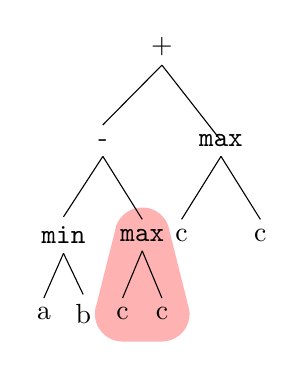
\begin{tikzpicture}[level distance=12mm]
\tikzstyle{level 1}=[sibling distance=15mm]
\tikzstyle{level 2}=[sibling distance=10mm]
\tikzstyle{level 3}=[level distance=10mm,sibling distance=5mm]


%\Tree [.+ [.- [.min a b ] c ] [.max c c ]]
\node (+) {+}
  child { node (-) {-}
    child { node (min) {\hmin}
      child {node (a) {a}}
      child {node (b) {b}}
    }
    child { node (max2) {\hmax}
      child {node (c4) {c}}
      child {node (c5) {c}}
    }
  }
  child { [sibling distance=5mm] node (max) {\hmax}
    child { node (c2) {c}}
    child { node (c3) {c}}
  };
\begin{pgfonlayer}{background}
\fill[red,opacity=0.3] \convexpath{c4,max2,c5}{10pt};
\end{pgfonlayer}
\end{tikzpicture}

&
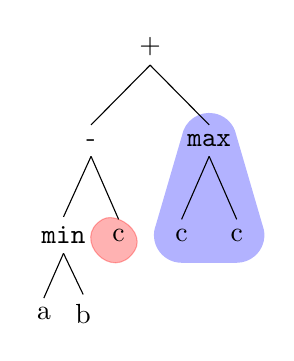
\begin{tikzpicture}[level distance=12mm]
\tikzstyle{level 1}=[sibling distance=15mm]
\tikzstyle{level 2}=[sibling distance=7mm]
\tikzstyle{level 3}=[level distance=10mm,sibling distance=5mm]
%\Tree [.+ [.- [.min a b ] c ] [.max c c ]]
\node (+) {+}
  child {  node (-) {-}
    child { node (min) {\hmin}
      child {node (a) {a}}
      child {node (b) {b}}
    }
    child { node (c) {c}}
  }
  child { node (max) {\hmax}
    child { node (c2) {c}}
    child { node (c3) {c}}
  };
\begin{pgfonlayer}{background}

\fill[blue,opacity=0.3] \convexpath{c2,max,c3}{10pt};
%\fill[red,opacity=0.3] \convexpath{c}{10pt};
\draw[red,fill=red,opacity=0.3](c.north) to[closed,curve through={($(c.north east)!1.0!(c.south east)$) .. ($(c.south west)!1.0!(c.north west)$)}] (c.north);

\end{pgfonlayer}
\end{tikzpicture}
&
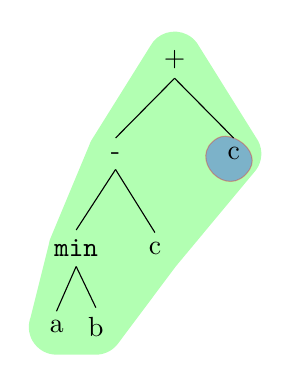
\begin{tikzpicture}[level distance=12mm]
\tikzstyle{level 1}=[sibling distance=15mm]
\tikzstyle{level 2}=[sibling distance=10mm]
\tikzstyle{level 3}=[level distance=10mm,sibling distance=5mm]
%\Tree [.+ [.- [.min a b ] c ] c ]
\node (+) {+}
  child { node (-) {-}
    child { node (min) {\hmin}
      child {node (a) {a}}
      child {node (b) {b}}
    }
    child { node (c) {c} }
  }
  child { node (c2) {c}};



  \begin{pgfonlayer}{background}
\fill[green,opacity=0.3] \convexpath{b,a,min,-,+,c2,c}{10pt};
\draw[red,fill=blue,opacity=0.3](c2.north) to[closed,curve through={($(c2.north east)!1.0!(c2.south east)$) .. ($(c2.south west)!1.0!(c2.north west)$)}] (c2.north);
\end{pgfonlayer}
\end{tikzpicture}
&
\vspace{0pt}
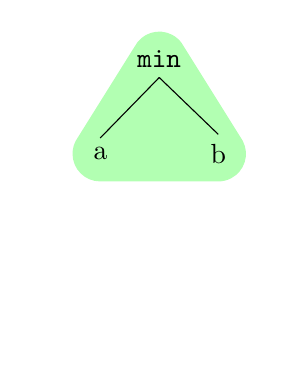
\begin{tikzpicture}[level distance=12mm]
\tikzstyle{level 1}=[sibling distance=15mm]
\tikzstyle{level 2}=[sibling distance=10mm]
\tikzstyle{level 3}=[level distance=10mm,sibling distance=5mm]
\node (min) {\hmin}
  child { node (a) {a}
     % [red,opacity=0.0]
    child {     [red,opacity=0.0] node (fake1) {f}
      child {    [red,opacity=0.0] node (fake2) {f}}
      child {    [red,opacity=0.0] node (fake3) {f}}
    }
    child {     [red,opacity=0.0] node (fake4) {f}
    [red,opacity=0.0]
    child { [red,opacity=0.0] node (fake) {f}}
    child { [red,opacity=0.0] node (fake2) {f}}
    }
  }
  child { node (b) {b}
     % [red,opacity=0.0]
    child {     [red,opacity=0.0] node (fake5) {f}}
    child {     [red,opacity=0.0] node (fake6) {f}}
  };
  \begin{pgfonlayer}{background}
\fill[green,opacity=0.3] \convexpath{a,min,b}{10pt};
\end{pgfonlayer}

\end{tikzpicture} \\
(i) & (ii) & (iii) & (iv)
\end{tabular}
\caption{We demonstrate the Halide rewriting algorithm using a TRS $R = \{\hmax(x, x) \rewrites x, (x - y) + y \rewrites x\}$ and an expression $\hmin(a,b) - \hmax(c,c) + \hmax(c,c)$. The algorithm attempts to simplify all subtrees bottom up; here, no rule applies to $\hmin(a,b)$ so it is not changed. Next (i), rule 1 rewrites $\hmax(c,c)$ to $c$. No rule applies to $\hmin(a,b) - c$, so we move to the rightmost subtree and rewrite again (ii) to obtain $c$ from $\hmax(c,c)$. Finally, we consider the entire tree $\hmin(a,b) - c) + c$ (iii) and apply rule 2 to produce $\hmin(a,b)$. No rules match this expression, so we are left with $\hmin(a,b)$ (iv).}
\label{fig:algoexample}
\end{figure*}

\section{Term Rewriting in Halide}
\label{sec:term-rewriting-in-halide}

The Halide compiler contains a term rewriting system composed of over a thousand
rules, operating over the space of Halide expressions\footnote{See Supplemental Material for
the full Halide expression grammar}.  \modified{The language of Halide expressions
operates over vectors and scalars of integers, booleans, and real values.  However, in
this work we concentrate on the TRS as it applies to integer and boolean values, for
both vectors and scalars, because the most important uses of the TRS within the compiler
apply to these types.  In this section, we give some background on term rewriting systems,
describe how the Halide compiler uses the TRS
and the design decisions that motivate the custom rewriting engine, as well as the scope
of our work.}

\subsection{Term Rewriting Systems}
Term rewriting systems~\cite{gorn1967} are sets of \textit{rewrite rules} used to transform expressions into a new form.  Such systems are widely
used in theorem proving~\cite{baader1999term} and abstract interpretation~\cite{cousot1977abstract, cousot1979systematic}.

Terms are defined inductively over a set of variables $V$ and a set of function symbols $\Sigma$. Every variable $v \in V$ is a term, and for any function symbol $f \in \Sigma$ with arity $n$ and any terms $t_1, ..., t_n$, the application of the symbol to the terms $f(t_1, ..., t_n)$ is also a term. (Constants are considered zero-arity functions.) We refer to the set of terms constructed from the variables $V$ and the function symbols $\Sigma$ as $T(\Sigma, V)$.

A \emph{rewrite rule} is a directed binary relation $l \rewrites r$ such that $l$ is not a variable, and all variables present in $r$ are also present in $l$ (i.e., $\mathcal{V}ar(l) \supseteq \mathcal{V}ar(r)$). A set of rewrite rules is a \emph{term rewriting system}.

Consider a set of terms $T(\Sigma, V)$ such that $\Sigma = \{\clubsuit, \diamondsuit\}$ and $V$ is an infinite set of variables. Let the term rewriting system $R$ consist of a single rule:

\[ R = \{ x_1 \clubsuit x_2 \rewrites x_1 \diamondsuit x_2 \} \]
We use $R$ to rewrite the term

\[ 
(y_1 \diamondsuit y_1) \clubsuit (y_2 \clubsuit y_3)
\]
The first step is matching; we find a substitution that will unify the left-hand side (LHS) of the rule with the term we are rewriting. Here, one possible substitution is:

\[
\{ x_1 \mapsto (y_1 \diamondsuit y_1), x_2 \mapsto (y_2 \clubsuit y_3) \}
\]
We then apply this substitution to the right-hand side (RHS) of the rule to obtain the rewritten version of the original term:

\[ 
(y_1 \diamondsuit y_1) \diamondsuit (y_2 \clubsuit y_3)
\]

\subsection{\modified{Uses of the TRS in Halide}}
\label{sec:uses-of-trs}
\modified{While the Halide compiler makes use of the TRS in numerous ways, the most important
  applications of the TRS are its uses as a fast simplifier and as a proof engine.  
  In many parts of the compiler, the TRS is used to rewrite expressions into simpler forms,
  which are easier for the compiler to reason about, and result in less code being generated for
  LLVM to consume at the backend.  Most importantly, the compiler uses the TRS to simplify expressions
  into constants or expressions monotonic with respect to loop bounds; these simplifications are core to Halide's
  ability to generate drastically different loop nests for different schedules.}

\modified{For example, consider the simple two-stage imaging pipeline $(g(x) = f(x - 1) + f(x) + f(x + 1)$.
  Halide enables programmers to fuse the computation of $f$ into $g$ at an arbitrary granularity
  using the \texttt{compute\_at} scheduling directive.  This requires Halide to automatically reason
  about which region of $f$ is required for a specific sub-region (or tile) of $g$, using interval
  arithmetic over symbolic values for the size of a tile of $g$.  For a tile size of 8, a tile of $g$
  is the region \texttt{[g.tile\_min, g.tile\_min+7]};  the region of $f$ required is
  \texttt{[g.tile\_min-1, g.tile\_min+8]}; and the number of values of $f$ to compute is then
  \texttt{g.tile\_min + 8 + 1 - (g.tile\_min - 1)}.  If the TRS can determine this is a static value
  of 10, the Halide compiler can then safely perform transformations requested by the user.  In this
  case, the compiler can use stack memory instead of inserting a dynamic allocation; or the loop can be
  completely unrolled; the loop can be vectorized; or $f$ can be mapped to GPU threads (since a single
  threadblock must have a compile-time-known size).  More generally, this kind of region analysis
  operates most effectively when the expressions are monotonic in the loop bounds; otherwise, interval
  arithmetic can result in vast overestimates of required regions.  These kinds of simplifications are essential
  for the compiler to work, and are usually not as simple as this example.}

\modified{The rules for simplifying to perform cancellations and
  ensure monotonicity are incredibly important for compiler
  performance. When we disabled all but the constant-folding rules to
  measure the importance of the simplifier, it was the absence of
  these specific rules that caused the (26.4$\times$) slow-down
  mentioned in Section~\ref{sec:introduction}. Without these rules,
  Halide is useless for high-performance image
  processing.}

%% Fodder from synthesis section:
%% For example, Halide relies on symbolic interval arithmetic to determine how much memory
%% to allocate and how many values to compute for each stage.  Symbolic interval arithmetic
%% is exact when an expression monotonically increases or decreases over a loop.}
%% For example, if $x \in [0, 100]$, then symbolic interval arithmetic states that
%% $\hmax(x, x/2 + 20) \in [20, 100]$, which is the tightest correct
%% bound; this bound is obtained by substituting in the lower and upper bounds of $x$
%% into the expression. However, in the presence of anti-correlated subexpressions
%% interval arithmetic becomes inexact, and is prone to overestimating
%% bounds. The expression $\hmin(x, 100 - x)$ when $x \in [0, 100]$ is bounded above by 50, but
%% symbolic interval arithmetic makes the weaker claim that it is bounded
%% above by 100, by setting the first instance of $x$ to 100 and the
%% second instance of $x$ to zero.

\modified{The use as a proof engine occurs when the compiler must prove properties about the code in order to guarantee the
  correctness of specific transformations or the relationships between bounds of
  different loops or producer-consumer relationships.  In such cases, the compiler constructs
  an expression that must be true or false in order to guarantee correctness, then applies
  the TRS to see if the expression simplifies to a single boolean value.}

\modified{For example, Halide uses Euclidean division, which rounds according to the sign of the
  denominator.  Lowering this to code requires emitting several instructions, which can be
  slower than native division.  When the compiler can statically prove the signs of the numerator
  and denominator, in some cases the code can be replaced by native division or even a different
  instruction altogether.  For example, for an expression \texttt{x / max(y, 1)} the compiler
  will try to prove $0 < \hmax(y, 1)$.  The TRS first invokes a rule to transform this to
  $0 < y || 0 < 1$, which then is transformed to true (since the second clause is always true).
  Thus, the compiler replaces the Euclidean division with machine division.}

\modified{TRS failures have adverse results on the compiler, making it flaky and
  difficult for programmers to use.  When the TRS fails to properly simplify an expression or
  prove a property, the consequences include: }
\begin{itemize}
\item Insufficiently tight bounds on loops and allocations, which may result in
  runtime failures (e.g. due to memory overallocation) or performance issues;

\item Failure of the compiler to apply optimizations, also resulting in slow performance;

\item Dynamic checks in the generated code for properties that could have been proven
  at compile time, leading to slower code;

\item Compilation failures, when the compiler is unable to correctly produce code
  even though the properties required hold, or when the proof engine itself crashes
  or loops infinitely.
\end{itemize}

Thus, correctness and generality of the TRS are essential to make the compiler
robust and able to generate fast code.

\subsection{Why a Custom Algorithm?}
\label{sec:whycustom}

\modified{In a term rewriting system, a single rule may be able to match an input expression in 
multiple ways, and there may be multiple rules in the ruleset which could be used 
to rewrite the expression. A term rewriting algorithm might choose one of many alternatives 
and later backtrack if it turns out not to be fruitful; it might make use of 
heuristics to choose a next step; it might exercise all the alternatives and keep 
the results in equivalence classes, as in an egraph. The Halide term rewriting algorithm
keeps only one expression in state and applies rules greedily, in a fixed priority.
This is very fast and requires very little memory; the tradeoff is that the algorithm 
may pick the ``wrong'' rule and have no way of undoing that decision. 
Since the rewriter is invoked many thousands of times with each call of the compiler, 
it chooses to sacrifice some solving power in exchange for performance.}

\subsubsection{\modified{Halide's Custom TRS Algorithm}}
\label{sec:customalgo}
The Halide term rewriting algorithm simplifies an input expression in a
depth-first, bottom-up traversal of the expression DAG. At each node, it 
uses the root node to pick a list of rules, then
attempts to match the subtree expression with the rule LHSs in a fixed priority. Matching
is performed purely syntactically, using C++ template metaprogramming.
 \modified{Halide rewrite rules contain special metavariables,
called \emph{symbolic constants}, that can match only with constant values; all other
variables can match any subterm as usual.}
When a match is found, the algorithm rewrites the
subtree expression using the RHS of that rule, and then attempts to simplify the
subtree expression again. If no rule matches the subtree, the traversal
continues; when the entire expression cannot be simplified further, the
rewritten expression is returned. See Figure~\ref{fig:algoexample} for a worked
example.

The rewrite rules optionally contain a compile-time predicate guard. 
These guards contain only symbolic constants\footnote{Existing 
rules sometimes have predicates that check if
  non-constant variables can be shown to have certain properties at compile
  time, but these are expensive and used sparingly.}; when the LHS of a rule
matches an expression, its guard is evaluated and only if it
is true will the rewrite be applied.

\modified{Halide rewrite rules are applied in a fixed priority, organized so that the TRS 
first attempts very basic rules such as constant folding, then tries more specific 
rules before more general ones. (We do not evaluate the current rule priority in this work.)}

\modified{Associativity and commutativity laws are particularly troublesome for term rewriting systems. 
For one expression $e$, the number of semantically equivalent expressions grows 
exponentially in terms of the number of AC operations $e$ contains. Some term rewriting 
systems perform a full \emph{AC matching} step during rewriting. Halide's TRS does not
perform this matching, but instead
includes multiple AC variations of rules.
However, a small number of Halide's rewrite rules have the effect of canonicalizing some commutative
expressions. (For example, if a commutative expression has a multiplication as its 
first operand and a subtraction as its second operand, a rule will switch their positions.)
These rules are all early in the application priority, so later rules can rely on
expressions having a quasi-canonical form.}

\subsubsection{Why Not Z3?}
\begin{table}
\caption{We compare the performance of Z3 and the Halide TRS in proving a set of 4304 expressions gathered from realistic compiler output.}
\begin{tabular}{l|r|r|r}
Tool & Runtime & Proven expressions & Not proven \\
\hline
Z3 & 7m29s & 1125 & 3179 \\
Halide TRS & 2s & 885 & 3419 
\end{tabular}
\label{tab:simplifiervsz3}
\end{table}


Given that we make use of the Z3 solver as an oracle for both verification and synthesis, it is natural to ask why Halide could not simply call Z3 for simplification. Z3 is the product of extensive development and is a very powerful, general-purpose solver. However, the Halide term rewriting system has a few key properties that Z3 does not: deterministic output, low memory and compute requirements, and domain-specific optimizations.

As discussed above, Halide compiler must return the same schedule every time the same pipeline is run. Z3 can fix a random seed, but long-running queries may complete on a more powerful server while timing out on a different machine.

\modified{While the Halide algorithm is less powerful than Z3, its deterministic, greedy rule application strategy
gives it a smooth performance curve, whether it succeeds or fails in simplifying an input expression. }
A solver like Z3 tends to give very good performance most of the time but gets bogged down in difficult cases, requiring the use of timeouts. The Halide algorithm ``fails fast'': on an input expression which does not match by any rule,  the Halide algorithm will complete in time linear to the size of the expression, taking on the order of one CPU cycle per term in the expression per rule in the TRS. To demonstrate this performance tradeoff, we gathered 4304 expressions from queries the Halide compiler made when compiling realistic pipelines, including provably true expressions and expressions not provably true. Z3 could prove more expressions true (within a 60 second timeout), but was starkly less performant. As shown in Table~\ref{tab:simplifiervsz3}, Z3 took over 7 minutes to check the set of expressions while the Halide TRS took just 2 seconds. The set of expressions is much smaller than the number of calls the compiler makes to the rewriter in compiling a single pipeline.

Because the Halide algorithm at every step chooses one rule to apply to the single expression it is working on, it scales well in terms of the number of rules in the TRS. See Section~\ref{ssec:compilationspeed} for an evaluation of the effects of adding newly synthesized rules on the performance of the compiler. 

Finally, although Z3 can simplify expressions, simply reducing the size of an expression is not necessarily the goal for the compiler. For example, gathering like terms in some cases can actually prevent Halide or LLVM optimizations from applying. The Halide rewriter uses a domain-specific strategy to guide expressions into more optimizable forms and can be changed or tuned as needed if further optimizations are discovered. 

\subsection{\modified{Completeness of the Halide TRS}}
\label{sec:completion}

\modified{We know by observation that the current Halide TRS cannot prove certain equalities 
that are in fact true, or reduce certain expressions that can be further simplified. 
Our goal is to learn new rules that would strengthen the TRS and allow it to make
further progress on these ``stuck'' expressions. This goal seems similar to that of 
\emph{completion}, which constructs a decision procedure through syntatic rewrites
for a set of identities. We do not use completion directly, although
our synthesis algorithm could be considered analogous to completion in some ways.}

\modified{In the standard Knuth-Bendix completion algorithm~\cite{knuth1983simple}, we take a
finite set of identities $E$ and a reduction order $>$ on terms as inputs; if successful, the
algorithm will return a finite, convergent set of rules $R$ that is equivalent to 
$E$. The algorithm may also fail, or fail to terminate. At each step the algorithm
maintains a set of identities and a set of rules, both of which can be updated; the 
algorithm may transform an identity into a new rule, find a new identity as a 
consequence of the ruleset, or use the present ruleset to refine either an identity 
or a rule. The algorithm runs until the ruleset has converged; specific implementations
may use some conditions under which to terminate with a failure.}

\modified{No finite set of identities exists for the theory of integers. We could
fix a set of identities to use in a completion procedure, but choosing these axioms
is a non-trivial task. One issue is that the theory contains axioms such as commutativity;
an identity such as $x + y \equiv y + x$ cannot be oriented by any possible reduction 
order, so our completion algorithm cannot make use of this fact. Another is that any
sufficiently powerful set of identities would almost certainly result in a non-terminating
completion procedure.  In addition, even if we use a subset of the Halide TRS for our
identities (thus yielding a confluent Halide TRS), our experience shows that many
failures in the compiler's use of the TRS are due to missing semantic facts that are not
derivable from the current Halide ruleset.}

%%% SAK: I integrated this into a sentence above.  Not sure we need this much text.
%% \modified{One approach might be to transform the existing Halide TRS into a set of undirected
%% identities $E_R$ and use it together with a reduction order as inputs to a completion procedure. 
%% If successful, this would yield a confluent TRS, for which any sequence of rewrites to 
%% an expression would ultimately yield the same result. (It is not immediately clear how 
%% to handle rule predicates in this case, however.) While this is certainly desirable, 
%% our experience is that many proof failures in the current Halide TRS is not due to a 
%% lack of confluence, but because of knowledge of the Halide expression langauge semantics 
%% not encompassed by the identities in $E_R$.}

\modified{%Instead, our synthesis algorithm seeks to learn rules which cannot (necessarily) be 
  %deduced from the existing ruleset.
In the absence of a finite set of identities, we
treat an SMT solver as an oracle for whether a suggested identity 
holds in our theory. If the identity holds and can be oriented using our reduction order, 
it is added as a rule. It is possible that the newly-synthesized rule may be a consequence 
of the existing ruleset and thus could have been found by running completion on $E_R$, 
but we know that many synthesized rules contain information that is previously 
unknown to the TRS.}

\modified{If we consider our solver as standing in for an infinite set of identities that make up
our theory, we clearly could synthesize an infinite number of rules. Here we make use
of the fact that expressions encountered by the compiler have some bias 
and are not sampled randomly from the entire expression space. In a preliminary 
experiment, we tried generating LHSs at random within a certain expression size and 
synthesizing RHSs to serve as new rules. We were able to find an extremely large number of 
``missing'' rules not represented in the current TRS, but the new ruleset had 
no measurable performance impact on benchmarks. Thus, we only synthesize rules if their LHS could be 
applied to at least one expression observed by the compiler under realistic usecases. %Even 
%without a formal definition of the bias on encountered expressions, we are able to 
%target synthesis to produce new rules that have some impact on compiler output.
}

\subsection{Scope: Robust, Fast, Non-Backtracking Ruleset}
\modified{In this work, we operate within the scope of Halide's TRS algorithm
  and work to make the TRS as correct, general, and robust as possible.  Because
  the space of expressions we consider constitutes an undecidable theory, a complete
  TRS is impossible.  Instead, we strive to improve correctness by ensuring the TRS
  will always terminate on any expression and that each individual rewrite
  preserves semantics; and we improve generality by expanding the ruleset to
  contain rewrites that apply to real-world expressions, rather than
  arbitrary new rules that may not apply to any expressions the compiler will encounter.}

\modified{These improvements require overcoming challenging obstacles.  First,
  we must perform a post-hoc verification of a large body of existing rules;
  proving a subset of rules correct or that a subset of rules do not result in infinite
  rewriting loops is insufficient to guarantee robust behavior.  Secondly,
  these rewrites operated in an undecidable theory, making automated verification
  difficult.  Finally, because of this undecidability, we cannot necessarily
  rely on traditional automated techniques to discover new rules.}
%\sak{Should we say something about how this applies to things other than Halide?}

\section{Soundness}
\label{sec:soundness}

We improve the Halide term rewriting system by ensuring its soundness in
two ways: first, we verify that each individual rule is correct, meaning that the
rewrite preserves semantics. Then we verify that the term rewriting system is
guaranteed to terminate on all inputs by ensuring that no sequence of
rule applications, on any input expression, can form a cycle.

\subsection{Rule Verification}
\label{sec:verification}
We verify each individual rule is correct by modeling Halide
expressions in SMT2 and using the SMT solver Z3~\cite{de2008z3} to
prove that the rule's left- and right-hand sides are equivalent. Most Halide expression
semantics map cleanly to SMT2 formulas. The functions \hmax and
\hmin are defined in the usual way, and \hsel in
Halide is equivalent to the SMT2 operator \texttt{ite}. Division and
modulo are given the Euclidean definitions in both Halide and
SMT2~\cite{boute1992euclidean}, though division and modulo by zero is handled
differently (in Halide both evaluate to zero).
%If a variable appears in the LHS of a rule as a divisor in a
%division or modulo operation, it is assumed to be non-zero. %The Halide
%expressions do not have a true boolean type (true and false are represented by
%unsigned integers of 1 bitwidth), so expressions must be typed as either
%\texttt{Int} or \texttt{Bool} when translated into SMT2. The Halide expression
Halide's TRS uses two vector-constructing operators, \texttt{broadcast} and \texttt{ramp}; all
other integer operators can be coerced to vector operators. 
\texttt{broadcast(x, l)} projects some value $x$ to a vector of length $l$; because of
the type coercion, we can simply represent \texttt{broadcast(x, l)} as the variable
\texttt{x} in SMT2. \texttt{ramp(x, s, l)} creates a vector of length $l$
whose initial entry has the value $x$ and all subsequent entries increase with
stride $s$. In SMT2, we represent this term as the symbolic expression $x + l *
s$, where $l$ must be zero or positive.

Given this modeling, for each rule, we assert any predicate guards are true, then
ask Z3 to search for a variable assignment that makes the LHS and RHS not
equivalent.  If Z3 indicates no such assignment exists, the LHS must be equivalent to
the RHS and the rule must be correct. We implemented an SMT2 printer for 
Halide rewrite rules that automatically constructs an SMT2 verification problem for each rule.
Rule verification using Z3 is fully automated
and can be run for the current set of rewrite rules used in the compiler via a script.

However, for 123
rules, Z3 either timed out or returned unknown. Nearly all of these rules used
either division or modulo. We used the proof assistant Coq to manually prove the
correctness of these remaining rules. In the course of these proofs, we
discovered we were also able to relax the predicate guards of \NumPredicatesRelaxed
rules; for example, in some cases a rule
with a guard requiring some constant to be positive would be equally valid
if the constant was non-zero.


\subsubsection{Evolving semantics}
\label{sub:evolvingsemantics}

This mostly-automated approach to verification assists with changing
the language semantics. Our initial work on verification was not on
the semantics described above: division or modulo by zero was originally
considered undefined behavior. Since we had already
modeled Halide semantics in SMT2, it was easy to alter the
definitions of division and modulo and re-run the verification scripts.
At the time of this second verification, there were
\NumZdivRules rules in the Halide TRS ruleset, and Z3 proved \NumZdivZThreeProvedRules
rules. We proved a further \NumZdivCoqProvedRules rules 
manually in Coq; since in the previous round all Coq proofs
included the assumption that all divisors were non-zero, in most cases
we had only to add a case to show that the rule was true when the
divisor was zero as well. In the course of reviewing
these proofs, we identified \NumZdivRelaxedPredicates rules whose
predicates included the condition that a divisor be non-zero and where
that condition could safely be lifted. We found that the remaining
\NumZdivFalseRules rules were not correct under the new semantics and
submitted a patch to amend them.

Overall results for verifying rule correctness are described in Section~\ref{sec:eval-correctness}.

\subsection{Termination}
\label{sec:termination}

\modified{Under the umbrella goal of simplifying expressions, the Halide TRS uses
many strategies: it may attempt to make expressions as short as possible; it may factor out
vector operations or more expensive operations such as division; it may attempt to
canonicalize subexpressions so they can cancel or be shown equivalent. These
strategies are not necessarily aligned and may even undo each other. Crafting new rules 
can thus require a detailed understanding of the ruleset and its various applications. 
In this section we formalize the Halide expression simplification strategy that was
previously only encoded in the ruleset itself. In doing so, we also prove that since 
each rule strictly makes progress in accordance to this strategy, the Halide TRS always terminates.}

Consider a term
rewriting system containing only one rule: $x + y \rewrites y + x$. The term
$3 + 5$ matches the LHS of the rule and is rewritten to $5 + 3$, which can again
be matched to the rule and rewritten to $3 + 5$, and so on. Termination failures in the Halide TRS have occurred in the past\footnote{See for example https://github.com/halide/Halide/pull/1525}, causing unbounded recursion and eventually a stack overflow in the compiler. This is tricky to debug, and may not always be reported by users, since the error is fairly opaque. To show that this type of error has been eliminated, we must prove that there is no expression in the Halide expression language that can be infinitely rewritten by some sequence of rules that form a cycle.

Intuitively, we can think of Halide expressions as existing in some multi-dimensional space; when an expression is rewritten by a rule, it moves from one point in that space to another. If each rule always rewrites expressions such that they move monotonically in some direction through the expression space, then no sequence of rules can form a cycle. These directions correspond to our intuition about why certain rules are useful (like the examples at the beginning of this section). We can consider each of these directions as a dimension in the expression space. If we formalize this desirable ordering and show that all rewrites from one expression to another strictly obey it, then we will have a proof of termination.

We provide this formalism and prove that the Halide term rewriting system must terminate by constructing a \emph{reduction order}, a strict order with properties that ensure that, for an order $>$ and a rule $l \rewrites r$, if $l > r$, then for any expression $e_1$ that matches $l$ and is rewritten by $l \rewrites r$ into $e_2$, it must be true that $e_1 > e_2$. Crucially, this order is evaluated over rule terms, and not over all expressions that those terms may match. We take the definition of a reduction order and the next two theorems from~\citet{baader1999term}.

\begin{theorem}\label{theorem:terminates}
A term rewriting system $R$ terminates iff there exists a reduction order $>$ that satisfies $l > r$ for all $l \rewrites r \in R$.
\end{theorem}

A reduction order is a strict order that must be well-founded, meaning that every non-empty set has a least element with regard to the order, to prevent infinitely descending chains. It must be \emph{compatible with $\Sigma$-operations}: for all expressions $s_1, s_2$, all $n \geq 0$, and all $f \in \Sigma$:
\[
s_1 > s_2 \implies f(t_1,...t_{i-1},s_1,t_{i+1},...,t_n) > f(t_1,...t_{i-1},s_2,t_{i+1},...,t_n)
\]
for all $i, 1 \leq i \leq n$ and all expressions $t_1,...t_{i-1},t_{i+1},...,t_n$. This property means that if a rewrite rule transforms a subtree in some expression $e$, the $>$ relation is preserved between the original expression $e$ and the rewritten expression $e'$. Finally, a reduction order is \emph{closed under substitution}: for all expressions $s_1, s_2$ and all substitutions $\sigma \in \mathcal{S}ub(T(\Sigma,V))$, 
$s_1 > s_2 \implies \sigma(s_1) > \sigma(s_2)$. When we match some left-hand side term $l$ to some expression $e$, we are defining a substitution for each of the variables in $l$ with some subtree in $e$; we then use that substitution to rewrite $e$ to $e'$. If our order is closed under substitutions, we know that for any expression we match to $l$, the resulting rewritten expression will obey the ordering.

Choosing a single monotonic direction in which to rewrite expressions would be overly restrictive. 
The Halide TRS is used both to prove expressions true and to simplify them; when using it as a prover, we want to put both sides of an equality into some normal form, but it doesn't particularly matter what that form is. When using the TRS to simplify expressions, on the other hand, reducing the size of an expression has important performance benefits. Since we need an ordering that covers the full Halide simplification strategy, we make use of the following theorem:

\begin{theorem}
The lexicographic product of two terminating relations is again terminating.
\end{theorem}

Thus, our strategy in finding a reduction order to cover the handwritten ruleset is to pick an order $>_a$ such that for all rules $l \rewrites r$, either $l >_a r$ or $l =_a r$. Then, we pick another order $>_b$ such that for all rules $l \rewrites r$ where $l =_a r$, either $l >_b r$ or $l =_b r$. We continue in this way until a sequence of orders has been found such that for their product $>_{\times}$, $l >_{\times} r$ holds for the entire ruleset.  Our final ordering consists of 13 component orders.

Many of our component orders are defined using a measure function that counts the number of particular operations or other features in a term. We say that $s > t$ when $s$ has more vector operations than $t$, then when $s$ has more division, modulo and multiplications operations, and so on. As a sample proof sketch of this flavor of order, consider an order $s_1 >_* s_2$ that holds when the number of multiplication operations is greater in $s_1$ than in $s_2$. We represent this through a measure function $|s_1|_*$ that returns the count of multiplication operations in $s_1$; since this function maps a term to a natural number, the order is clearly well-founded. The order is also compatible with $\Sigma$-operations; we compute our measure function as follows:


\[
|f(t_1,...,t_n)|_* = \sum_i^n |t_i|_* + \begin{cases} 1 & \textrm{if } f = * \\
                                                      0 & \textrm{otherwise}
                                        \end{cases}
\]

It clearly follows that given $|s_1|_* > |s_2|_*$, it must be true that:

\[
|f(t_1,...t_{i-1},s_1,t_{i+1},...,t_n)|_* > |f(t_1,...t_{i-1},s_2,t_{i+1},...,t_n)|_*
\]

To ensure the order is closed under substitution, we need to add one more constraint. Imagine a rule $x * 2 \rewrites x + x$. Although there are fewer $*$ symbols in the righthand term than on the left, that would not be true for a substitution $\sigma = \{x \mapsto (z * z)\}$. We add a condition that for every variable present in $s_1$, it must occur either fewer or an equal number of times in $s_2$. With this constraint there is no possible substitution that increases the value of the measure function in $s_2$ that would not result in an increase by an equivalent or greater amount in $s_1$. This gives us the order:

\[
s_1 >_* s_2 \textrm{ iff } |s_1|_* > |s_2|_* \wedge \forall x \in \mathcal{V}ar(s_1) . |s_1|_x \geq |s_2|_x
\]

Most of the component orders in the full reduction order take the form above. These orders guarantee termination no matter what sequence rewrite rules are applied to an expression. However, for part of the existing ruleset, we were obliged to take into account the order in which rules are applied in the Halide TRS algorithm.

For example, one existing rule is the canonicalization $(c_0 - x) + y \rewrites (y - x) + c_0$ where $c_0$ is a constant. If $y$ is also a constant, this rule forms a cycle with itself, and could not possibly obey any reduction order. Fortunately, the rule immediately before it in the TRS handles that specific case ($((c_0 - x) + c_1 \rewrites fold(c_0 + c_1) - x)$), so by this sort of non-local reasoning we know that $y$ is not a constant, and therefore the rule strictly decreases a measure which counts the number of constants on the right-hand side of an addition.

%The handwritten ruleset had many rules that eliminated the occurrence of a variable, such as $x + x \rewrites x * 2$. It seems natural to define an order based on the measure function $|s_1|_x$, but for a substitution $\sigma = \{x \mapsto 3\}$, $|3 + 3|_x \not > |3 * 2|_x$. However, the simplifier algorithm always attempts constant folding before any other rule, so we know that the rule $x + x \rewrites x * 2$ can only be invoked if $x$ is not a ground term.

%Similarly, we have several rules that factor out an occurrence of a variable and introduce the constant 0 into the expression. We define an order on the occurrences of the constant 0 by defining a measure function that takes the count of terminals or leaves in the expression and subtracts the count of the constant 0; if terms $s_1$ and $s_2$ have the same number of leaves, but more of the leaves of $s_2$ are the constant 0, then $s_1 > s_2$.

%\[
%s_1 >_0 s_2 \textrm { iff } |s_1|_{leaf} - |s_1|_0 > |s_2|_{leaf} - |s_2|_0 \wedge |s_1|_{leaf} = |s_2|_{leaf} \wedge \forall x \in \mathcal{V}ar(s_1) . |s_1|_x \geq |s_2|_x
%\]

% For the rule $\texttt{max}(x + y, x) \rewrites \texttt{max}(y, 0) + x$, the order will not hold for the substitution $\sigma = \{x \mapsto 0\}$. However, we know the rule $0 + x \rewrites x$ will be invoked before this one, so the rule cannot be evaluated on the expression $\texttt{max}(0 + y, 0)$.

Relying on non-local reasoning makes our order more brittle; if the simplifier algorithm were to be changed, the termination guarantee could be lost. However, we use only a small number of basic rules in this way, which are unlikely to be changed.

Besides giving a termination guarantee, the reduction order is necessary if we want to synthesize new rewrite rules. If we do not constrain newly-synthesized rules to obey a consistent reduction order with the existing human-written ones, they form cycles with the existing rules and cause infinite recursion in the TRS. Additionally, the reduction order is the formal encoding of the types of transformations we find desirable, so the reduction order limits synthesis to rules that rewrite expressions in a useful direction.

In constructing the reduction order, we found 8 rules that contradicted a desirable ordering, and submitted patches to either delete or modify them. With this amendment, the reduction order can be shown to hold over the entire Halide ruleset, and the guarantee of termination is complete. To ensure this guarantee is preserved, we build a script that automatically checks the full set of rules in the compiler to ensure they respect the reduction order. A full description of the reduction order is given in the supplemental material.




\section{Increasing Completeness: Synthesizing Rewrite Rules}
\label{sec:completeness}
%\jln{Possible TODO: I refer to expressions from the corpus we learn from as input expressions throughout. If anyone has a 
%better suggestion please let me know.}
\begin{figure*}
%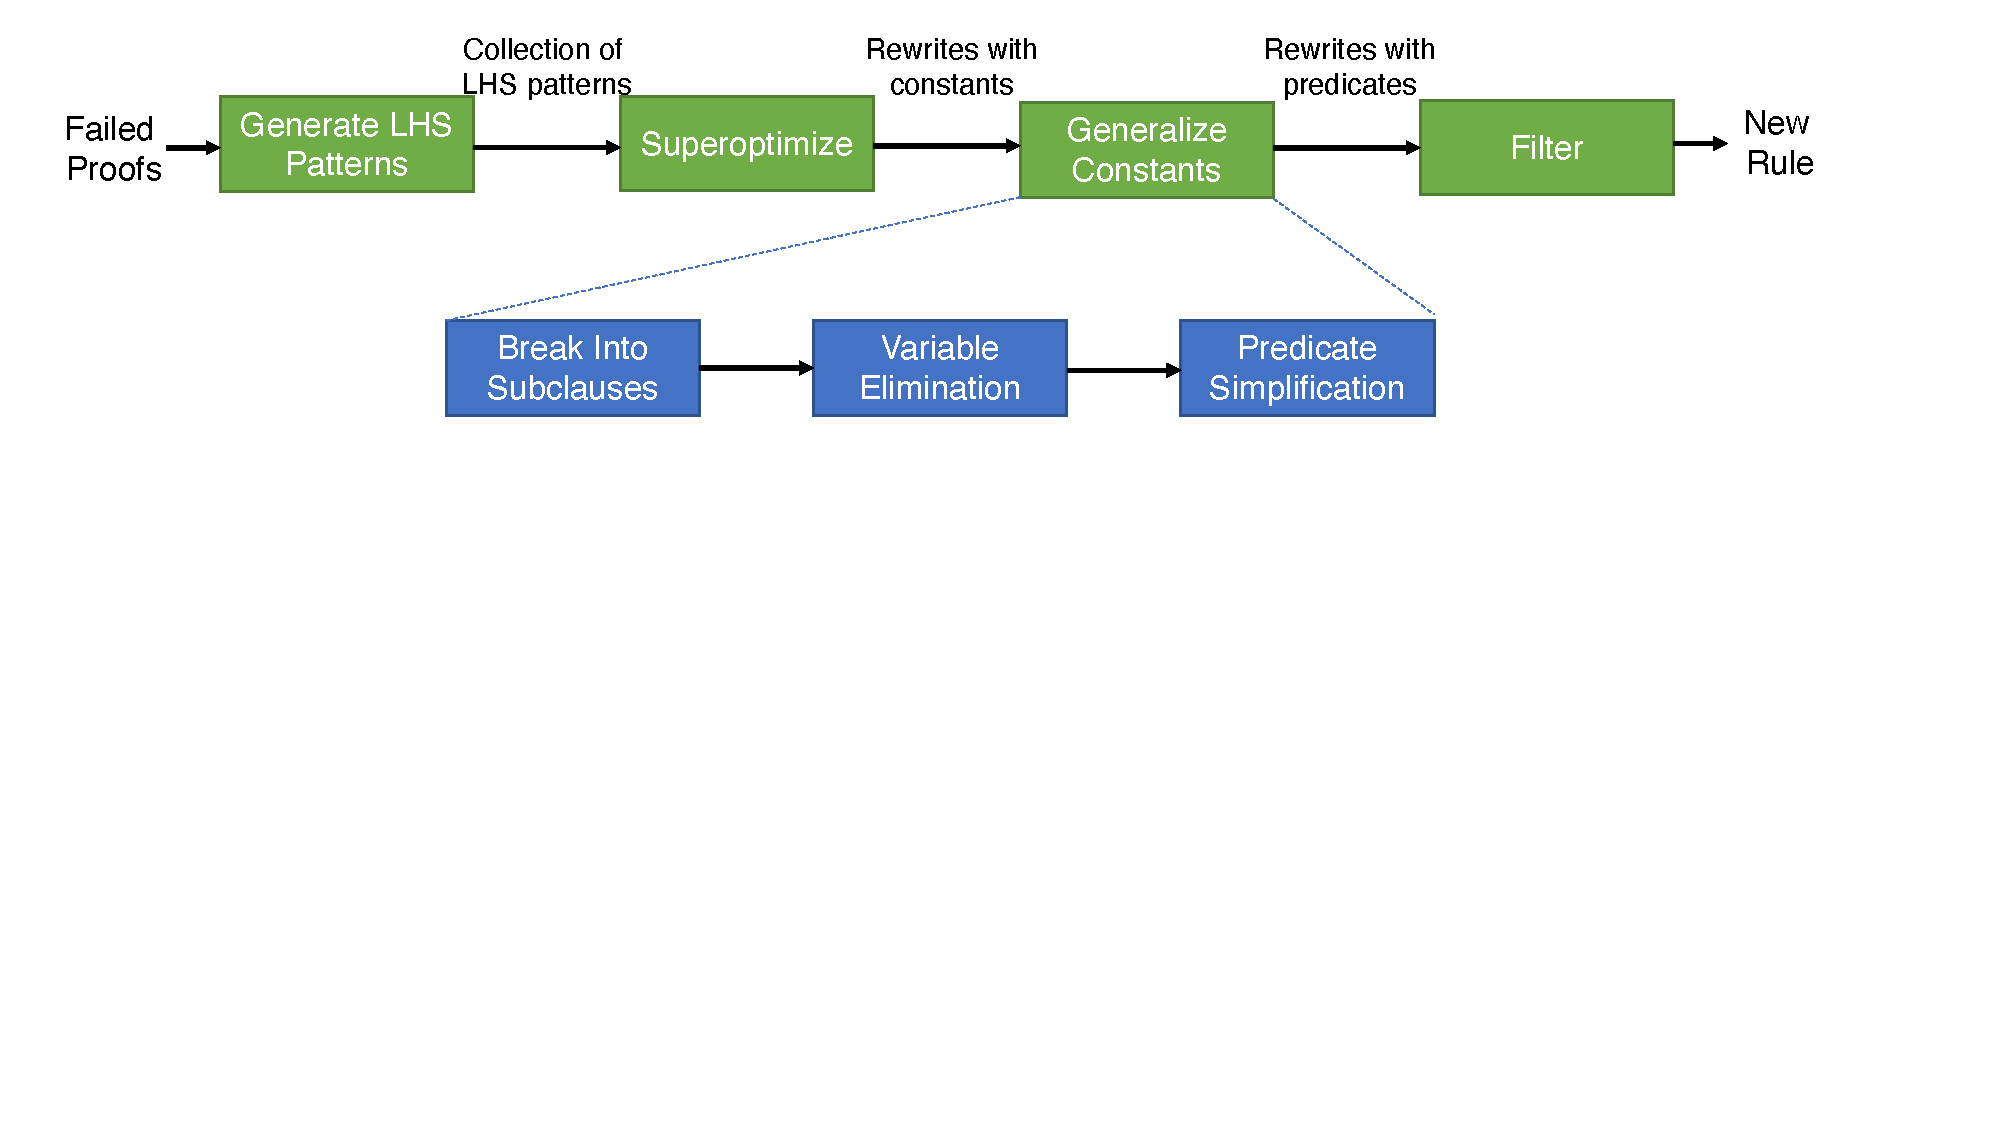
\includegraphics[width=1.\columnwidth,natwidth=610,natheight=642]{figures/synthesis-flow.pdf}
%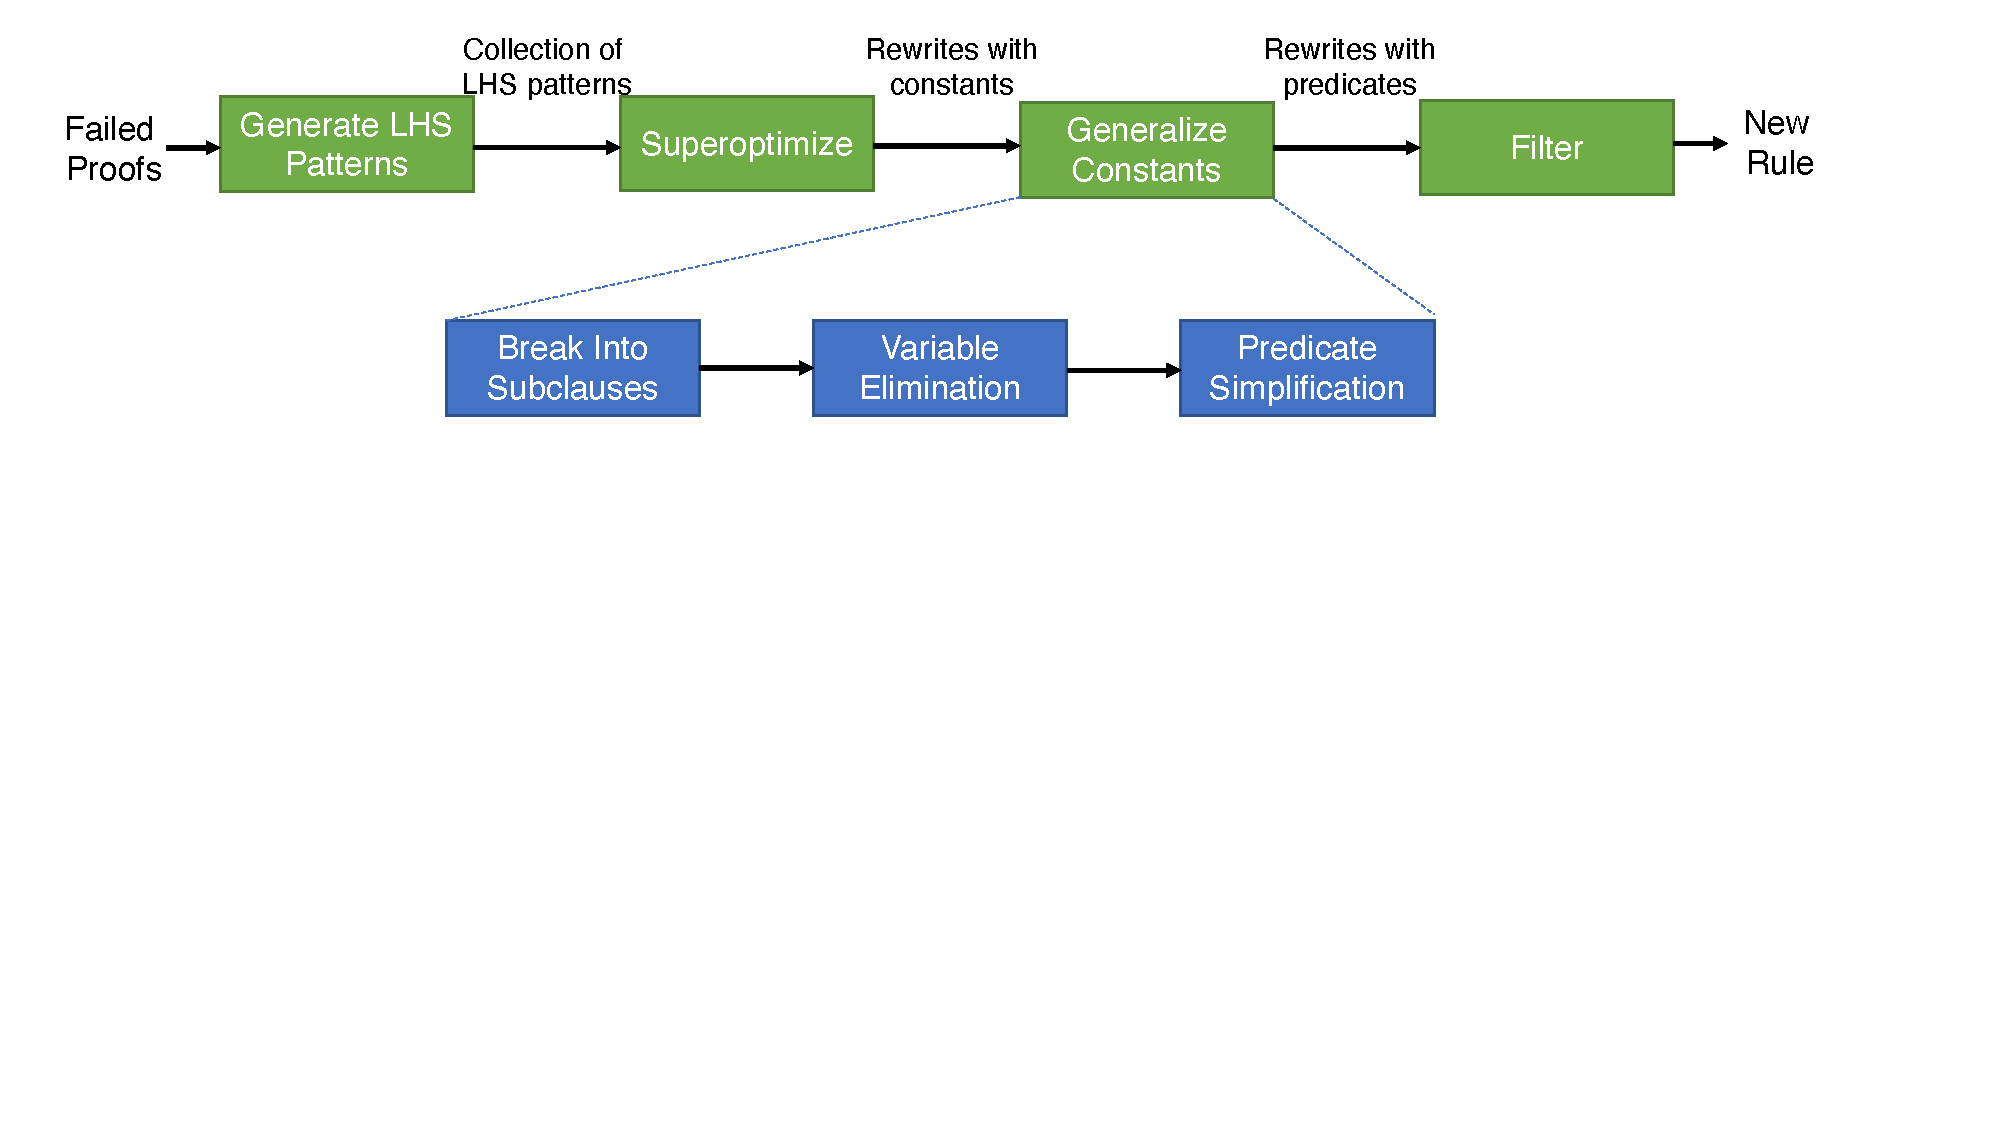
\includegraphics[width=1.\columnwidth]{figures/synthesis-flow.pdf}

% x_1 < select(x_2, c_0, c_1) + x_1 -> !x_2

  \tikzstyle{stage}=[fill=blue!10, draw=none, minimum height=3em, minimum width=11em]
  \tikzstyle{example}=[fill=orange!10, draw=none, minimum height=3em, minimum width=23em]
  \tikzstyle{label}=[fill=blue!10, draw=none, minimum height=3em, minimum width=1em]
  \begin{tikzpicture}[node distance=1.5cm,auto,>=latex']
    \node (s1) [stage] {\shortstack{Input expression}};
    \node (s2) [stage] [below of=s1] {\shortstack{Generated LHS\\patterns (Fig.~\ref{fig:lhspatterns})}};
    \node (s3) [stage] [below of=s2] {\shortstack{AC matching\\(Sec.~\ref{sec:rhsacmatching})}};
    \node (s4) [stage] [below of=s3] {\shortstack{Superoptimized with\\CEGIS (Sec.~\ref{sec:rhssynthesis})}};
    \node (s5) [stage] [below of=s4] {\shortstack{With symbolic\\constants (Sec.~\ref{sec:generalizing-constants})}};
    \node (s6) [stage] [below of=s5] {\shortstack{Substitute concrete\\values of $x_i$}};
    \node (s7) [stage] [below of=s6] {Candidate predicate};
    \node (s8) [stage] [below of=s7] {\shortstack{Verify or find new\\counterexample}};
    \node (s9) [stage] [below of=s8] {Rule with predicate};
    \node (s10) [stage] [below of=s9] {Add variants (Sec.~\ref{sec:filtering})};
    \node (l1) [label] [left of=s1,node distance=6em] {(a)};
    \node (l2) [label] [left of=s2,node distance=6em] {(b)};
    \node (l3) [label] [left of=s3,node distance=6em] {(c)};
    \node (l4) [label] [left of=s4,node distance=6em] {(d)};
    \node (l5) [label] [left of=s5,node distance=6em] {(e)};
    \node (l6) [label] [left of=s6,node distance=6em] {(f)};
    \node (l7) [label] [left of=s7,node distance=6em] {(g)};
    \node (l8) [label] [left of=s8,node distance=6em] {(h)};
    \node (l9) [label] [left of=s9,node distance=6em] {(i)};
    \node (l10) [label] [left of=s10,node distance=6em] {(j)};    

    \draw [line join=miter] (l8.west) -- ([xshift=-1em] l8.west) -- ([xshift=-1em] l6.west) -- ([xshift=-0.9em] l6.west) node {};
    \path[->] ([xshift=-1em] l6.west) edge node {} (l6.west);
        
    \path[->] (s1) edge node {} (s2);
    \path[->] (s2) edge node {} (s3);
    \path[->] (s3) edge node {} (s4);
    \path[->] (s4) edge node {} (s5);
    \path[->] (s5) edge node {} (s6);
    \path[->] (s6) edge node {} (s7);
    \path[->] (s7) edge node {} (s8);
    \path[->] (s8) edge node {} (s9);
    \path[->] (s9) edge node {} (s10);                

    \node (e1) [example] [right of=s1,node distance=19em]
          {$(y + 2) < \hsel(u < z, -3, 4) + (y + 2)$};
    \node (e2) [example] [right of=s2,node distance=19em]
          {\shortstack{
              \color{darkgray}
              \tiny{$\ldots$} \\
              \color{darkgray}
              \tiny{$(x_1 + 2) < x_2 + (x_1 + 2)$} \\
              $x_1 < \hsel(x_2, -3, 4) + x_1$ \\
              \color{darkgray}
              \tiny{$\hsel(x_1 < x_2, -3, 4)$} \\
              \color{darkgray}
              \tiny{$\ldots$}}};
    \node (e3) [example] [right of=s3,node distance=19em]
          {\shortstack{No reassociated/commuted variants \\ match an existing rule.}};
    \node (e4) [example] [right of=s4,node distance=19em]
          {$x_1 < \hsel(x_2, -3, 4) + x_1 \rightarrow \boxed{\neg x_2}$};
    \node (e5) [example] [right of=s5,node distance=19em]
          {$x_1 < \hsel(x_2, c_0, c_1) + x_1 \rewrites \neg x_2$};
    \node (e6) [example] [right of=s6,node distance=19em]
          {\shortstack{
              $0 < \hsel(false, c_0, c_1) + 0 = \neg false ~ \wedge$ \\
              $1 < \hsel(false, c_0, c_1) + 1 = \neg false ~ \wedge$ \\
              $0 < \hsel(true, c_0, c_1) + 0 = \neg true$ 
          }};
    \node (e7) [example] [right of=s7,node distance=19em]
        {$0 < c_1 \wedge c_0 \le 0 $};
    \node (e8) [example] [right of=s8,node distance=19em]
        {\shortstack{
            $\exists~ x, c ~s.t.~ (0 < c_1 \wedge c_0 \le 0) ~\wedge$ \\
            $(x_1 < \hsel(x_2, c_0, c_1) + x_1 \neq \neg x_2)$ ? \\
            No solutions. Predicate is sufficient.
        }};
    \node (e9) [example] [right of=s9,node distance=19em]
          {$x_1 < \hsel(x_2, c_0, c_1) + x_1 \rewrites \neg x_2 \pred 0 < c_1 \wedge c_0 \le 0 $};
    \node (e10) [example] [right of=s10,node distance=19em]
          {\shortstack{
              $x_1 < \hsel(x_2, c_0, c_1) + x_1 \rewrites \neg x_2 \pred 0 < c_1 \wedge c_0 \le 0 $ \\
              $x_1 < x_1 + \hsel(x_2, c_0, c_1) \rewrites \neg x_2 \pred 0 < c_1 \wedge c_0 \le 0 $
          }};



    \path[->] (e1) edge node {} (e2);
    \path[->] (e2) edge node {} (e3);
    \path[->] (e3) edge node {} (e4);
    \path[->] (e4) edge node {} (e5);
    \path[->] (e5) edge node {} (e6);
    \path[->] (e6) edge node {} (e7);
    \path[->] (e7) edge node {} (e8);
    \path[->] (e8) edge node {} (e9);
    \path[->] (e9) edge node {} (e10);

  \end{tikzpicture}
  \caption{Overall flow of the synthesis pipeline (in blue) with worked example (in orange). (a) We harvest expressions from real compilations on which the TRS could make no further progress. (b) We enumerate all sub-trees of these to generate left-hand sides that would match each expression. Our example will focus on one such pattern. (c) We obtain a right-hand side by first checking if any reassociated or commuted variants of it match an existing TRS rule. (d) If not, we superoptimize the pattern using CEGIS. (e) This rule is specific to the particular values of any constants that appear. We then replace any constants with new variables $c_0, c_1, etc.$ to obtain a more general version of the rule. We must now synthesize a sufficient condition on these new variables under which the rule still holds. (f) To do this, we treat the rewrite as an equality and take the conjunction over a set $S$ of different values for the non-constant variables $x_0, x_1, etc.$. (g) Simplifying the result gives a candidate predicate. This is a \emph{necessary} condition. (h) We then check if it is also \emph{sufficient} condition using Z3. (i) If a counterexample is found, we add these new values of $x$ to $S$ to obtain a new candidate predicate and repeat until we have a sufficient condition to serve as our predicate. (j) Finally, we construct variants of the rule in which the LHS has been commuted.}
\label{fig:synthesis-flow}
\end{figure*}


\modified{Although the Halide term rewriting system is necessarily incomplete, we can strengthen 
it by finding expressions on which the TRS can no longer make progress and creating 
rules that will further simplify them.
In this section, we describe a workflow for automatically augmenting the Halide TRS with new rules.}

\modified{Given an \emph{input expression} that the TRS failed to simplify, our goal is to find a rule that
can rewrite it. A high-level view of the synthesis pipeline is shown in Figure~\ref{fig:synthesis-flow}.
%and Algorithm~\ref{alg:synthesis-algorithm} shows the corresponding pseudocode.
We begin with an expression we will attempt to further simplify; 
first, we synthesize rules that contain concrete constants from the input expression. 
Next we generalize those rules by replacing constant values with symbolic constants and synthesizing compile-time 
predicate guards 
that check the validity of the rule on the values matched by the symbolic constants. If we 
find such a rule, we know that adding it to the TRS will enable it to simplify the input
expression as well as any similar expressions it may encounter.}

\paragraph{Gathering input expressions}
The set of input expressions may come from a bug report, or may be gathered from compiler logs. With logging enabled, the compiler records two
kinds of problematic expression for which new TRS rules may be helpful:
\modified{non-monotonic expressions, which can result in over-conservative
bounds for loops and memory allocations; and proof failures,
which may prevent Halide from performing certain optimizations
(see Section~\ref{sec:uses-of-trs}). 
Of course, absent an oracle, it is difficult to know if the TRS has fully simplified 
some expression or if it lacks the solving power to continue simplification. 
When the TRS is used as a proof engine, its goal is to reduce an expression to true.
In this case, we can fuzz-test failed proofs by assigning all variables in an expression
random values and evaluating; if we cannot find an assignment that evaluates to false,
the expression may indeed be reducible to true, so we log it as an input expression.}


\begin{figure*}
\begin{tabular}{lll}
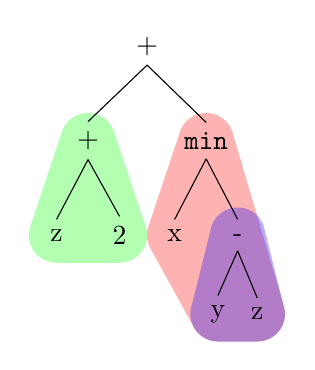
\begin{tikzpicture}[level distance=12mm,baseline=(current bounding box.center)]
\tikzstyle{level 1}=[sibling distance=15mm]
\tikzstyle{level 2}=[sibling distance=8mm]
\tikzstyle{level 3}=[level distance=10mm,sibling distance=5mm]

% tried to label subtrees but positioning looks weird, fix later
\node (+) {+}
  child { node (+2) {+}
    child { node (z) {z}  } % edge from parent node[left,draw=none] {$v_1$}
    child { node (2) {2} }}
  child { node (min) {\hmin}
    child { node (x) {x}}
    child { node (-) {-} %edge from parent node[right,draw=none] {$v_2$}
      child {node (y) {y}}
      child {node (z1) {z} } % edge from parent node[right,draw=none] {$v_3$}}
    }};


\begin{pgfonlayer}{background}
\fill[red,opacity=0.3] \convexpath{x, min, z1, y}{10pt};
\fill[blue,opacity=0.3] \convexpath{y, -, z1}{10pt};
\fill[green,opacity=0.3] \convexpath{z, +2, 2}{10pt};
\end{pgfonlayer}
\end{tikzpicture} &
\begin{tabular}{llll}
$(z + 2) + \hmin(x, y - z)$ & $\hmin(x, y - z)$ & $z + 2$ & $y - z$ \\
$v_1 + \hmin(x, y - z)$ & $\hmin(x, v_2)$ & & \\
$v_1 + \hmin(x, v_3)$ & & & \\
$(z + 2) + \hmin(x, v_3)$ & & & \\
$v_1 + v_2$ & & &
\end{tabular}
\end{tabular}
\caption{Given the input expression $e = (z + 2) + \hmin(x, y - z)$, we find all possible 
LHS patterns by substituting fresh variables for subterms, for all valid combinations. Then, we repeat the process for 
each individual subterm. This process yields the list of candidate LHS terms on the right.}
\label{fig:lhspatterns}
\end{figure*}

\subsection{Generating LHS Patterns}

\modified{
  Our first step is to find LHS terms that could match the input expression, or any portion of it. 
We can enumerate all such terms through a kind of inverse matching.
When we rewrite an expression with a rule, 
we match the expression to the rule's LHS by finding a substitution for all variables in
the LHS that will unify it with the input expression. Here, we start with an input expression,
then fix a substitution by mapping some of its subterms to fresh variables. We 
replace those subterms with the new variables, constructing a term that can 
be matched with the input term.
If we perform this inverse matching for all sets of subterms, we find \emph{all possible LHSs} that could match the
input expression. 
When a subterm occurs more than once in the input expression, we construct a LHS that 
use the same variable to replace it in multiple places and LHSs that replace its
occurrences with different variables.
We repeat the procedure on all \emph{subterms} of the input expression.  The result is the set of all 
LHSs that match any part of the input expression. See Figure~\ref{fig:lhspatterns} for a worked example. }

\modified{This number of LHSs is exponential in the size of the input expression, so we use a few heuristics to narrow 
our search. We bound the size of candidate LHSs to have seven or fewer leaves, since longer terms are less likely to 
result in rules general enough to justify inclusion in the ruleset. 
Additionally, since we process input expressions in batches, we remove 
duplicate LHSs as well as LHSs that differ only in the values of their constants. 
Finally, we have found it helpful to keep a blacklist of LHSs for which we previously
failed synthesize rules; for example, $v_1 + v_3$ 
cannot form a rule, so we filter it out as a candidate.}

\subsection{Synthesizing Right-Hand Sides} 
\label{sec:synthesizing-candidate-rules}
\modified{%
Given a candidate left-hand side, we attempt to 
synthesize a right-hand side that is semantically equivalent and
respects the reduction order, namely $\mathit{LHS} > \mathit{RHS}$.
We employ two strategies for synthesizing right-hand sides:
delayed AC matching, and counter-example guided inductive synthesis (CEGIS) of 
the RHS followed by synthesis of the rule predicate guard.} 

\subsubsection{Finding Right-Hand Sides through AC matching}
\label{sec:rhsacmatching}
\modified{The first strategy reflects the Halide design decision not to perform any AC matching in the TRS, for efficiency reasons. 
Instead, AC matching is effectively performed during rule synthesis, by checking whether the LHS could be 
rewritten by the existing TRS after a suitable application of associativity and commutativity laws to the LHS. 
To this end, we generate all possible reassociations and commutations of the candidate LHS term and pass them to the existing TRS. 
If any of them can be simplified, we create a new rule that rewrites 
the original, untransformed LHS term to the result of the simplification.  Note that this result may include applications of more than one rewriting step, so the new rule is not merely an AC-variant of an existing rule. }

\modified{For example, assume our TRS includes the rule $(x + y) - x \rewrites y$, 
and let $((u + 2) + v) - u$ be a candidate LHS term. The rule does not match the candidate but it matches its variant $(u + (v + 2)) - u$, rewriting it to the result $v + 2$. The candidate and the result give us the rule $((u + 2) + v) - u \rewrites v + 2$. }
\jln{QUESTION: Any suggestions to clarify this figure?}

\begin{center}
\begin{tabular}{ccccccccccccccc}
$($ & $x$       & $+$ & $y)$ & $-$ &  $x$ &                                     & $(x$      & $+$ & $y$       & $)$ & $-$ &  $x$ &             & \\
$($ & $(u + z)$ & $+$ & $v)$ & $-$ &  $u$ & $\xrightarrow[\text{AC}]{\text{}}$  & $(u$      & $+$ & $(z + v)$ & $)$ & $-$ &  $u$ & $\rewrites$ & $z + v$ 
\end{tabular}
\end{center}





\modified{We can consider this procedure a kind of lazy, offline AC matching, because if the Halide TRS 
performed full AC matching while rewriting expressions, it would be able to apply the rule $(x + y) - x \rewrites  y$ to the candidate expression $((u + 2) + v) - u$ after reassociating it to $(u + (v + 2)) - u$, obtaining the result $v + 2$.  Delaying AC matching to synthesis has the effect of restricting the system to a single, offline round of AC and memoizing the result in the form of a new TRS rule if we are successful. 
Note that the synthesis procedure below could have found this rule, but checking for AC
variants of existing rules is far cheaper. About three quarters of our synthesized rules are generated by this method.}

\subsubsection{Finding Right-Hand Sides through Synthesis}
\label{sec:rhssynthesis}
\modified{If the first method fails, we apply CEGIS to superoptimize the left-hand side pattern.
In superoptimization~\cite{massalin1987superoptimizer}, we take a program and search 
for an equivalent program within some grammar that is preferable according 
to some cost function. Here our grammar is that of the Halide expression language, 
the method for testing program equivalence is the Z3 solver, and we use the node
count of the programs as a proxy for our full reduction order.}

\modified{Similar to prior work in superoptimization~\cite{regehr2018superoptimization, mangpo2016superoptimization},
we search the expression space for a RHS using a CEGIS loop. This loop alternately calls Z3 as a
verifier, which checks if a candidate RHS is equivalent to the LHS on all inputs, 
and a learner, which finds a candidate RHS that is equivalent to the LHS on
a limited set of inputs.
We begin by choosing a single-op
RHS and ask the verifier if it is equivalent to the LHS. If it is not, we get back 
a counterexample of assignments to the variables for which the right- and left-hand side are 
not equivalent, which we keep as a set of test inputs. 
We then ask the learner for a new RHS that is equivalent to the LHS 
only on the counterexample assignments we found in the last step. 
If we cannot find an equivalent single-op sequence,
we iteratively increase the number of operations, ensuring we find shorter sequences
first.  If CEGIS returns a sequence semantically equivalent to the LHS pattern with fewer
operations, we use it together with our LHS to form a candidate rule.}

\modified{ The learner portion of the CEGIS loop creates a candidate RHS
  %expression from a parameterized bytecode
  %sequence of fixed size that is fed to an interpreter. Each bytecode
  %instruction takes parameters that select between the possible operators and
  %operands available to it. Thus,
  %this bytecode
  %sequence serves as an SSA representation of an expression tree. The
  %interpreter is evaluated abstractly on symbolic inputs to produce a
  %sketch~\cite{DBLP:conf/aplas/Solar-Lezama09, torlak2014lightweight}, 
  %capable of acting as any Halide expression in our
  %search space depending on the bytecode values. The learner uses Z3
  by creating a sketch~\cite{DBLP:conf/aplas/Solar-Lezama09, torlak2014lightweight}
  that consists of a small bytecode interpreter that encodes the possible
  operations and operands the RHS can use, along with a bound on the number of instructions.
  The learner uses Z3 to query for a sequence of bytecodes within the bound, that, when
  run through the interpreter, is semantically
  %solve for the bytecode values that makes the sketch semantically
  equivalent to the LHS over the test inputs. If a solution is found,
  substituting the produced bytecode values into the sketch
  and applying the TRS reduces it to a concrete candidate RHS. One
  complication arising from this approach is that a bytecode sequence
  of a fixed number of ops may produce expression trees of a larger
  size if intermediate values are reused. We reject any such solutions
  in a post-pass by checking each synthesized RHS against the LHS
  using the full reduction order. An alternative solution would be
  introducing let bindings into our search space so that the size of
  the expression tree could be bounded by the number of ops in its SSA
  form. However, we could not identify any significant rewrite rules
  lost to this filtering, so we deemed this an unnecessary
  complication. }

While Z3 is a powerful tool for synthesis, there are certain types of expressions 
containing division or modulo that Z3 nearly always fails to reason about during the CEGIS process. (We experimented with the SMT solvers Yices2~\cite{jovanovic2017solving} and MathSAT5~\cite{mathsat5}, but were not able to obtain appreciably better results.)
Z3 is better able to reason about expressions containing concrete constants, rather than
universally quantified variables, so we synthesize rules using candidate LHSs with 
concrete constants from the input expression and generalize them later.
We limit the use of division and modulo in our op-codes to be division
or modulo by 2 only, and rely on the generalization step described next to
widen the set of denominators for which a rule applies.  Because of this
restriction, our synthesized rules cannot contain non-constants in denominators
or the right-hand side of a modulo.  As a result, our synthesis system cannot
construct all rules a human can.

\begin{table*}
\caption{Sample rules synthesized by our process. }
\small
\begin{tabular}{l|l|l}
LHS & RHS & Predicate \\
\hline
$(x*y) - (z + (w*x))$ & $(x*(y - w)) - z $ & \\
$x < (y + x) + z$ &  $0 < (y + z)$ & \\
$\hmax(x*x, y) + \hmax(z, w*w) < c_0$ & false & $c_0 <= 0$ \\
$\hsel(x, c_0, y) < \hmin(\hsel(x, c_1, y), c_2)$ & false & $\hmin(c_1, c_2) <= c_0$ \\
$\hmin((x + ((y - x)/c_0)*c_0) + c_1, y)$ & $y$ & $1 <= c_1 \wedge -1 <= (-1/c_0)*c_0 + c_1$ \\
\end{tabular}
\label{tab:samplerules}
\end{table*}

\subsection{Generalizing Constants and Finding Predicate Guards}
\label{sec:generalizing-constants}

\modified{If either AC-matching search (Section~\ref{sec:rhsacmatching}) or CEGIS-based synthesis (Section~\ref{sec:rhssynthesis}) were successful, 
we now have a candidate rewrite
rule that contains concrete values originating from the input expression.
To generalize the rule, we replace such constants with fresh \emph{symbolic constants} 
and synthesize a guard that is true when the rule is valid. 
Recall that in the Halide TRS, a variable in the LHS matches any subterm, while a 
symbolic constant matches only a constant value (see Section~\ref{sec:customalgo}); the guards, which are predicates over symbolic constants, can thus be evaluated at compile time. }

\modified{Our goal is to generalize the equality by synthesizing a guard predicate $\phi$ 
over the symbolic constants in the LHS and RHS terms such that our rule is valid whenever
$\phi$ evaluates to true: }
\[ \forall \vec{c} \forall \vec{x} \;.\; \phi(\vec{c}) \implies LHS(\vec{x},\vec{c}) = RHS(\vec{x},\vec{c})
\]

\modified{First, we check to see if this condition is satisfied when $\phi$ is 
always true. If it is, then no predicate guard is needed. Otherwise, we need 
to synthesize an expression for $\phi$. We find candidates for $\phi$ iteratively 
by first choosing a small set of values $S$ for the variables 
in $\vec{x}$ and finding the candidate guard $\phi_S$. We check to see if $\phi_S$
is a sufficient predicate guard for all $\vec{x}$; if it is not, we add
counterexamples to the set $S$ and repeat.}

\[ \forall \vec{c} \forall \vec{x} \in S \;.\; \phi_S(\vec{c}) \implies LHS(\vec{x},\vec{c}) = RHS(\vec{x},\vec{c})
\]

\modified{We initialize $S$ with all basis vectors, which are 
values $\vec{x} = ( 0, \ldots, 0, 1, 0, \ldots, 0 )$ that include exactly one unit value,
plus the zero vector.  
We then unwind the right-hand side of the implication and substitute in the concrete values 
from $S$ to get:}

\[ \forall \vec{c} \forall \vec{x} \in S \;.\; \phi_S(\vec{c}) \implies (LHS(\vec{x_1},\vec{c}) = RHS(\vec{x_1},\vec{c}) \wedge \ldots \wedge
LHS(\vec{x_k},\vec{c}) = RHS(\vec{x_k},\vec{c}))
\]

\modified{We use the Halide TRS itself to simplify the conjunction on the right-hand side of the
implication. Since all occurrences of $\vec{x}$ have been replaced with concrete
values, we get back an expression that contains only symbolic constants, which we
use as our candidate guard $\phi_S$. }

\modified{We test whether $\phi_S$ is sound on all $\vec{x}$. }
\[ \exists \vec{c} \; \exists \vec{x} 
   \;.\; LHS(\vec{x},\vec{c}) \not= RHS(\vec{x},\vec{c})
\]

\modified{If this query has a solution $\vec{x}$, then the guard is unsound.  
If so, we add the counterexample $\vec{x}$ to $S$, and construct a new guard $\phi_S$.  
We repeat this process for several iterations (four, in our experiments) and if 
we fail to find a sound guard, we switch to an alternative strategy that converts 
the current (unsound) candidate $\phi_S$ to disjunctive normal form and tests
each clause in turn to check if it is a sufficient guard.
If it is, that clause becomes the guard.  If no clause is sound, we discard the rule.
If the loop terminates with Z3 timing out or returning ``unknown'', we return
the current $\phi_S$, flagging it for human attention as requiring a manual proof. 
We exclude all such cases from our experiments.}


\modified{As an example, consider the candidate rule:}
%
\[ x_0 < \hsel(x_1, c_0, c_1) + x_0 \rewrites \neg x_1
\]
\modified{We initialize $S$ with three basis vectors $\{(0,\mathit{false}), (0,\mathit{true}), (1,\mathit{false})\}$ and construct $\phi_S$:}
%
\begin{equation*}
\begin{split}
 \phi_S(\vec{c}) \iff 
 &  \forall_{\vec{x} \in S} \;.\; LHS(\vec{x},\vec{c}) = RHS(\vec{x},\vec{c}) \\
 \iff & 
 0 < \hsel(\mathit{false}, c_0, c_1) + 0 = \neg\mathit{false} \; \wedge \\
                                                   & 0 < \hsel(\mathit{true}, c_0, c_1) + 0 = \neg \mathit{true}  \; \wedge \\
                                                   & 1 < \hsel(\mathit{false}, c_0, c_1) + 1 = \neg\mathit{false}
\end{split}
\end{equation*}

\modified{Simplifying the RHS with the TRS, we obtain $\phi_S$: }
%
\[  \phi_S(\vec{c}) \iff 0 < c_1 \wedge c_0 \le 0
\]
Next we check whether $\phi_S$ is sound for all $\vec{x}$.  It is, so we have a completed rule:

\[ x_0 < \hsel(x_1, c_0, c_1) + x_0) \rewrites \neg x_1 \;\pred \;0 < c_1 \wedge c_0 \le 0
\]


\subsection{Adding Rule Variants}
\label{sec:rulevariants}
\modified{Once we have a generalized rule with a valid predicate, we eagerly compensate for the lack
of AC matching in the Halide TRS by adding AC variants of the rule as well. We find 
all commuted variants of the rule's LHS,
with respect to the partial commutative canonicalization as described in Section~\ref{sec:customalgo}.
 (This is exponential in the size of the number 
of commutative operators, which is tractable given our bounds on LHS term size). 
Then, we find all reassociations of the rule's right-hand side. For each variant LHS, 
we choose a RHS variant by serializing expressions to strings and finding the RHS 
that has the shortest edit distance from that LHS. }

\modified{For example, the LHS of the first rule below has four additions and can be commuted 
to 16 variants. The RHS of the rule can be reassociated in two different ways. For the 
commuted variant of the LHS on the second line, we choose the other means of reassociating
the RHS as it has a smaller edit distance.}

\begin{equation*}
\begin{split}
(x + (y - ((z + (w + x)) + u))) & \rewrites y - (z + (w + u))) \\
(y - (((w + x) + z) + u)) + x & \rewrites y - ((z + w) + u)
\end{split}
\end{equation*}

\modified{The intuition is that there is no a priori reason 
to prefer one reassociated variant to another; they are almost certainly equal in 
terms of our reduction order. Thus, we choose the RHS that perturbs the structure of the 
LHS as little as possible, in order to avoid rewriting common subexpressions in the hopes
of canceling them out later.}


\subsection{Filtering Rule Output}
\label{sec:filtering}
\modified{As a final step, we check each output rule for redundancy with the rule batch found
by the synthesis pipeline. For each new rule, we check
that no earlier rule has precisely the same LHS and predicate; if so, it can be discarded.
Then, we check that no earlier rule is more general than the current rule: a rule is more 
general than another if they have similar LHSs, but a variable appears in the first rule 
in a place where the second rule has a more specific subterm, or if they have the same LHS
but the predicate of the first rule implies the predicate of the second.}

Finally, we
check that the candidate rule obeys our reduction order in order to
preserve our termination guarantee. If the candidate rule passes these
filters, and the predicate has not been flagged for human review, the
rule can be added to the TRS ruleset automatically without any human
auditing.

\section{Evaluation}
\label{sec:evaluation}

% (1186-367)/1186
\newcommand{\PercentPossibleToSynth}{69\%}
\newcommand{\NumRulesInCorrectnessExperiment}{321}
\newcommand{\PercentRulesResynthesized}{58\%}

In evaluating the benefits of the verifier and synthesizer, we answer the following questions:

\begin{itemize}
  \item \textbf{Does the synthesizer produce better rules than a human expert?} The TRS has been manually extended five times in response to bug reports pointing out limitations of the compiler. We synthesized these five rulesets automatically and found that the human-authored rules were less general and in one case were incorrect. (Section~\ref{sub:bugfixes})
  \item \textbf{Can verification contribute to the Halide TRS, or is testing alone sufficient?} Although handwritten rules have been extensively fuzz-tested and new rules are peer-reviewed before inclusion, we were still able to discover 5 unsound rules through verification. In addition, verification was able to identify 44 rules that needed to be changed after a significant semantics redefinition, which would have been challenging to discover through testing. (Section~\ref{sec:eval-correctness})
  \item \textbf{What is the best way to use synthesis and verification in development?} We survey several cases from recent Halide development where human experts used the synthesis machinery as an assistant, finding that this hybrid model is more powerful than either the human developer or the synthesizer alone. (Section~\ref{sub:synthassistant})
  \item \textbf{Can synthesis be used for large-scale improvements of the TRS?} We gather a corpus of over 100,000 expressions on which the TRS can make no progress and iteratively synthesize rules using the corpus as input. We synthesize 4127 rules and add them to the TRS ruleset without a human audit. We find that the enhanced ruleset reduces peak memory usage in compiled code, sometimes dramatically, in 197 of our benchmarks. We also find no significant compile-time slowdown even with this 4.5-fold increase in ruleset size. (Section~\ref{sub:endtoendexperiment})
  \item \textbf{Could the entire TRS have been synthesized?} Encouraged by the large-scale experiment, we ask how far we are from being able to bootstrap the entire TRS automatically---something that we considered too ambitious originally. First, we find that \PercentPossibleToSynth~of the existing ruleset are accessible to our current synthesizer in principle; the remaining rules contain operators not yet supported by the tool. % or cannot be reasoned about automatically by our solver. 
  We test the synthesizer's power by removing \NumRulesInCorrectnessExperiment{} accessible rules from the original ruleset one by one and attempting to synthesize a replacement, successfully finding a replacement rule \PercentRulesResynthesized{} of the time.  We find this encouraging for future applications of the synthesizer. (Section~\ref{sub:replacementexperiment})
\end{itemize}

We discuss these findings in more detail below, grouping them into three sections. First we examine bug reports from Halide’s past and evaluate whether the machinery presented in this paper could have fixed them automatically. Second, we examine cases where beta versions of our verifier and synthesizer assisted humans in both fixing bugs and also correctly making larger changes to the compiler. Third, we fuzz the compiler to mine for issues that could be fixed with new simplifier rules, and automatically fix them before they ever appear as a bug in a real program. In this way we demonstrate that this machinery would have been useful in the past, is useful in the present, and will help avoid entire classes of bugs in the future.

%\jln{don't forget to do this!}
%Note for reviewers: For the purposes of this anonymous submission, we will refer to code changes by letter, with corresponding diffs found in supplemental material. In this final version of the paper these will be replaced with GitHub issue and pull request IDs with links to Halide’s GitHub page.

\subsection{Comparing the Synthesizer to Human-Authored Rules}

\subsubsection{Does the synthesizer produce better rules than a human expert?}
\label{sub:bugfixes}

%We expect a human expert to create rules that are as general as possible while also including rules that take advantage of less general situations, such as when special cases allow stronger rewrites.  Can a synthesizer produce rules that are both general and expressive? 

%We compared synthesized rules against five sets of rules added manually. We have found that the expert wrote rules that were less general than the synthesized rules, and in some cases were incorrect. Additionally, the synthesizer avoided adding a specialized rule because the TRS could already achieve its effect with rules present in the TRS. We discuss in Section~\ref{sec:limitations} the limitations of when the synthesizer cannot achieve such general rules. 

% AA: I found the two paragraphs above redundant with the summary we just gave in the itemized list.


% A) https://github.com/halide/Halide/pull/3719
% B) https://github.com/halide/Halide/pull/3761
% C) https://github.com/halide/Halide/pull/3765
% D) https://github.com/halide/Halide/pull/3770
% E) https://github.com/halide/Halide/pull/3780
% F) https://github.com/halide/Halide/pull/4721
% G) https://github.com/halide/Halide/pull/4772
% H) https://github.com/halide/Halide/pull/4439
% I) https://github.com/halide/Halide/pull/4850 


We searched through Halide’s change history and selected the five pull requests that addressed issues by adding new rewrite rules to Halide’s TRS. These pull requests occurred before the Halide developers started routinely using the verifier and synthesizer when changing the TRS. \modified{These can be found as summarized diffs $\mathbb{A}$-$\mathbb{E}$ in supplemental material, or in their original form on the Halide project website
\footnote{
$\mathbb{A}$: \url{https://github.com/halide/Halide/pull/3719}
$\mathbb{B}$: \url{https://github.com/halide/Halide/pull/3761}
$\mathbb{C}$: \url{https://github.com/halide/Halide/pull/3765}
$\mathbb{D}$: \url{https://github.com/halide/Halide/pull/3770}
$\mathbb{E}$: \url{https://github.com/halide/Halide/pull/3780}
}}
. Creating these rewrite rules as a human is an amount of work disproportionate to the size of the change. The author of the rules must prove them correct on paper, and a second reviewer must check their work. As we will see, bugs can slip through despite this review. 

In each case we take the test expressions committed as part of the change and feed them to our synthesizer to see if it would have produced the same rewrite rules as the humans did. In cases where humans did not check in tests for their new rules, we wrote our own. In total, across these five cases humans added 24 new rules. The synthesizer generated 42, covering all but one of the human rules, while correcting and generalizing others. In cases $\mathbb{A}$, $\mathbb{C}$, and $\mathbb{E}$, the rules generated by the synthesizer are an exact match to the human-generated rules. In case $\mathbb{B}$ the synthesizer matched the human but also crafted 8 commuted variants of the human rules, making them more widely applicable. As an example, for the human-written rule:

\[
\hmax(\hmax(x, y) + c_0, x) \rewrites \hmax(x, y + c_0) \pred c_0 < 0
\]

The synthesizer produced effectively the same rule, along with a variant:

\begin{align*}
& \hmax((\hmax(x, y) + c_0), x) \rewrites \hmax((y + c_0), x) \pred c_0 \leq 0 \\
& \hmax(x, (\hmax(x, y) + c_0)) \rewrites \hmax(x, (y + c_0)) \pred c_0 \leq 0
\end{align*}

Case $\mathbb{D}$ is the most interesting. It contains four rules involving comparisons of min and max operations. What happened for each was identical, so we will only discuss the min rules. The first rule is:

\[
\hmin(x, c_0) < \hmin(x, c_1) + c_2 \rewrites \hfalse \pred c_0 \geq c_1 + c_2)
\]

This rule is incorrect (consider $c_0 = c_2 = 1$, $x = c_1 = 0$). It can be fixed by adding the term $c_2 \leq 0$ to the predicate. The synthesizer produced the correct version of this rule, along with two generalizations of it:

\begin{align*}
& \hmin(x, c_0) < \hmin(x, c_1) + c_2 \rewrites  \hfalse \pred c_2 \leq 0 \wedge c_1 + c_2 \leq c_0 \\
& \hmin(x, c_0) < \hmin(x, y) + c_1 \rewrites c_0 - c_1 < \hmin(x, y) \pred c_1 \leq 0 \\
& \hmin(x, c_0) < \hmin(y, x) + c_1 \rewrites c_0 - c_1 < \hmin(y, x) \pred c_1 \leq 0
\end{align*}

The second human rule was:
\[
\hmin(x, c_0) < \hmin(x, c_1) \rewrites \hfalse \pred c_0 \geq c_1
\]
The synthesizer found a more general rule, along with three other commuted variants (elided for space):
\[
\hmin(x, y) < \hmin(x, z) \rewrites y < \hmin(x, z)
\]
Any expression which matches the human-written rule would also match the synthesized one. The synthesized version does not simplify to the constant “false” in a single step. However, after applying this rule to the case considered by the human, we get $c_0 < \hmin(x, c_1)$ where $c_0 \geq c_1$. The simplifier then reduces this to “false” in a second step, so the human-written rule becomes unnecessary. The synthesizer considered the human-written rule, but discarded it as less general than the one above.

Case $\mathbb{D}$ also included the rewrite rule: 
\[
x \% x \rewrites 0
\]
which was the sole rule the synthesizer could not generate, as we did not include modulo by non-constants in our CEGIS interpreter.

With this one exception, across these five code changes the synthesizer generated more general, more correct rules than the humans, and would clearly have been a useful assistant to the Halide developers if they had had it at the time.


\subsubsection{What fraction of the Halide rules could have been synthesized?}
\label{sub:replacementexperiment}
To bootstrap a TRS, we could start with a TRS equipped with a basic set of rules and synthesize the remaining rules as the TRS encounters expressions needing those rules.  How far is the synthesizer from supporting this ambitious vision?

Given the space of possible rewrites explored by the synthesizer, we believe that it can currently produce at most \PercentPossibleToSynth{} of rules that exist in the current TRS. The obstacles to synthesizing all human-written rules include (i)~the inability to automatically verify some rules or preconditions (see Question 3 above); (ii)~lack of support for some operators in our synthesizer. 

We tested the synthesizer's ability to recreate the original ruleset in the following experiment. We instrumented the ruleset to associate expressions from compilations of Halide's correctness test suite with individual rules invoked when those expressions are rewritten. We gathered a set of rules for which we had at least three expressions that matched the rule, and filtered out those rules that are out of scope for the current synthesizer, because their right-hand sides contain operators we do not support. This gave us a set of \NumRulesInCorrectnessExperiment{} rules. For each of these rules, we disabled the rule in the TRS, then used its matching expressions as input to the synthesizer. The synthesizer was able to find rules in 186 cases, or about \PercentRulesResynthesized{} of the rules. Of the other 135 cases, in 43 of them other rules in the existing TRS happened to combine to rewrite the specific input expression even without the target rule; for example, this often occurred when the matching expression contained combinations of constants that could be exploited by other rules. 10 of the 92 failure cases were due to timeouts in the synthesis process, while 15 specifically failed to synthesize a predicate. Given that it was difficult to target the desired rule precisely, we find these results to be a promising state of the technology.


\subsection{Practical Uses of the Synthesizer and Verifier}

\subsubsection{Can verification contribute to the Halide TRS, or is testing alone sufficient?}
\label{sec:eval-correctness}

The Halide TRS has a stringent development process: new rules are peer reviewed after they are proven on paper, and fuzzing has been discovering bugs for months. It is thus reasonable to ask whether mechanized verification can add any value. Our verification discovered five new soundness bugs and 17 instances of rules whose predicates were overly restrictive. The former bugs eluded the fuzzer; the latter are deemed too hard so the fuzzer does not look for them. Furthermore, because the verification infrastructure was in place, it was possible to verify a change of semantics without much additional effort, identifying 44 rules that were incorrect under the new semantics.

The first use of verification took place when the TRS had not yet been merged into the Halide master branch. We ran the verification pipeline and discovered three incorrect rewrite rules, listed in Table~\ref{tab:verfirstround}. The rules that could not be checked with Z3 were proved true using the Coq proof assistant (none of the manually proved rules were found to be incorrect). While these bugs were found automatically the fixes were performed by hand, as the synthesis pipeline did not yet exist. 

\jln{check that the body of this footnote doesn't occur on a page before the number does}
Case $\mathbb{H}$
\footnote{
\label{footnote:casesfi}
$\mathbb{F}$: \url{https://github.com/halide/Halide/pull/4721}
$\mathbb{G}$: \url{https://github.com/halide/Halide/pull/4772}
$\mathbb{H}$: \url{https://github.com/halide/Halide/pull/4439}
$\mathbb{I}$: \url{https://github.com/halide/Halide/pull/4850}
}
is a change to the semantics of Halide that may not have even been attempted without the verifier. In this change, Halide defined division or modulo by zero to evaluate to zero, instead of being undefined behavior, in response to an issue discovered by Alex Reinking~\cite{reinkingthesis}. Existing tests and real uses of Halide were useless as a test of this change, as \emph{they were all carefully written to never divide by zero}. Within the TRS, this change required rechecking every rewrite rule that involves the division and modulo operators. Whereas previously each rule assumed that a denominator on the LHS could not be zero, now it was necessary to either show that the rule was still correct in the case where a denominator was zero, or constrain the rule to only trigger when the denominator was known to be non-zero. This was done by encoding the new semantics into the verifier, and reverifying all rules. Because division and modulo is involved, these rules cannot always be mechanically verified. 141 rules were reverified with a human in the loop by revisiting and modifying existing Coq proofs. The mechanical re-verification was all but push-button; the manual effort for updating the Coq proofs was non-trivial, but about half of the effort of writing the original proofs from scratch. In this process, 44 existing rules were found to be incorrect in the new semantics and fixed. (Two of them were in fact not related to division, but were instead the first discovery of the bugs injected in case $\mathbb{D}$ above.) The remaining 42 rules were modified to only trigger when the denominator was known to be non-zero, either by adding a predicate to the rule, or by exploiting the TRS’s ability to track constant bounds and alignment of subexpressions. Three examples of now-incorrect rules were:

\begin{align*}
(x/y)*y + x\%y \rewrites & x \\
  -1 / x \rewrites & \hsel(x < 0, 1, -1) \\
(x + y)/x \rewrites & y/x + 1
\end{align*}

The first was modified to:
\[
(x/c_0)*c_0 + x\%c_0 \rewrites x \pred c_0 \neq 0
\]
and the other two were constrained to only trigger when the denominator is known to be non-zero via other means.

The cases discussed in Section~\ref{sub:bugfixes} all concern fixing existing problems while not introducing new ones. By giving a proof of soundness, showing that the ruleset is correct and that the rules are cycle-free, we also remove two entire classes of future bugs. For reference, over the life of the Halide project there have been 14 pull requests that fix incorrect rules, and 3 pull requests that modify rules in order to avoid cycles. Fixing a reduction order also guarantees that no new cycles can be introduced as long as new rules obey this order; without such a guide, it is possible to introduce a rule that would close a loop in some sequence of existing rule applications and cause a cycle, resulting in infinite recursion during compilation. 

\begin{table*}
\caption{Rules corrected through the first round of verification.}
{\renewcommand{\arraystretch}{1.2}
\begin{tabular}{r|l|l}
& Rule & Counterexample \\
\hhline{=|=|=}
Wrong &  $\frac{x * c_0}{c_1} \rewrites \frac{x}{(c_1 / c_0)} \pred c_1 \% c_0 = 0 \wedge c_1 > 0$ & $c_0 = -1, c_1 = 2, x = 1$\\
Fixed & $\frac{x * c_0}{c_1} \rewrites \frac{x}{(c_1 / c_0)} \pred c_1 \% c_0 = 0 \wedge c_0 > 0 \wedge \frac{c_1}{c_0} \neq 0$ & \\
\hhline{=|=|=}
Wrong & $(\frac{x + c_0}{c_1})*c_1 - x \rewrites x \% c_1 \pred c_1 > 0 \wedge c_0 + 1 = c_1$ & $c_0 = 2, c_1 = 3, x = -5$\\
Fixed & $(\frac{x + c_0}{c_1})*c_1 - x \rewrites (-x) \% c_1 \pred c_1 > 0 \wedge c_0 + 1 = c_1$ & \\
\hhline{=|=|=}
Wrong & $x - (\frac{x + c_0}{c_1})*c_1 \rewrites -(x \% c_1) \pred c_1 > 0 \wedge c_0 + 1 = c_1$ & $c_0 = 2, c_1 = 3, x = -5$\\
Fixed & $x - (\frac{x + c_0}{c_1})*c_1 \rewrites ((x + c_0) \% c_1) + (-c_0) \pred c_1 > 0 \wedge c_0 + 1 = c_1$ & \\

\end{tabular}
}
\label{tab:verfirstround}
\end{table*}

\subsubsection{What is the best way to use synthesis and verification in development?}
\label{sub:synthassistant}

% Is the expert equipped with the synthesizer better at developing rules than either the expert alone or the synthesizer alone? The synthesizer can accelerate rule development because it is correct by construction and also faster than a human expert. On average, the expert needed about 30 minutes to develop a rule, including a paper proof and the code review. Our synthesizer typically produces a batch of ten (verified) rules in about 5 minutes.

We have found that human experts can best leverage the strengths of the synthesis tool by using it as an assistant: for example by synthesizing a rule and then generalizing or simplifying it by hand, or by writing a rule and asking the tool to synthesize a valid predicate. Most importantly, this avoids committing new bugs, but it also accelerates rule development. Halide developers report that adding new rules by hand takes about 30 minutes per rule starting from sample input expressions through final review. Starting from the same input expressions, the synthesis tool can produce a batch of 10 verified rules in about 5 minutes.

Here we survey some cases from recent Halide development where the synthesis machinery was used in this way. \modified{The diffs are available as $\mathbb{F}$ through $\mathbb{I}$ in supplemental material or on the Halide project website\textsuperscript{\ref{footnote:casesfi}}.}

In case $\mathbb{F}$ a Halide developer encountered expressions that seemed like they could be simpler while working on real code, and rather than inventing a rule from scratch searched the logs of the synthesizer project for a known-correct synthesized rule that handled the case in question. This added four new rules that are variants of:
\[
\hmax(y, z) < \hmin(x, y) \rewrites \mathit{false}
\]
In case $\mathbb{G}$ a developer wrote 24 new rules, proving them on paper, and then checked their work by resynthesizing the predicates using the synthesizer, ensuring that the synthesized predicates agreed with the human’s and that those predicates were as broad as possible. Here the synthesis machinery served as a reviewer of rules rather than an author. Eight of these rules were in fact manual rederivations of the synthesizer’s output on case $\mathbb{D}$ above. The remaining 16 are generalizations that add constant terms. One example:
\[
\hmin(y + c_0, z) < \hmin(y, x) \rewrites \hmin(z, y + c_0) < x \pred c_0 < 0
\]

Halide endeavors to be a safe language, meaning that certain things are checked at compile time or runtime rather than being undefined behavior. In case $\mathbb{I}$, Halide was changed such that instead of asserting that no output value has a dependency on any out-of-bounds input values, it now asserts the stricter condition that no out-of-bounds loads occur on the input, even if those loaded values cannot possibly affect an output.

This is a harder thing for the compiler to check, and analysis often conservatively found that it was possible for code to read out of bounds, when in fact it would not. The Halide developers ameliorate this in part by minimizing the number of non-monotonic expressions using aggressive simplification. In total 59 new rewrite rules were added as part of this change. Eight of these were synthesized automatically by copy-pasting a non-monotonic expression from a bug report into the synthesis machinery. Another 28 came from generalizing those rules by hand and then verifying the result. Twenty more were written by hand and then verified. Finally, there were three rules that could not be verified, because they involve the interaction of division and modulus. During this process a large number of bugs were found in human-written early versions of these rules. We found that with the verifier and synthesizer in hand, humans work quickly and rely on the machinery to catch their mistakes.

Generalizing from these four cases, we have found that having the verifier and synthesizer available as tools reduces the number of bugs committed, uncovers and fixes old bugs, and helps developers work more quickly by not only mechanizing correctness checking but also by synthesizing correct code. We also found that the guarantees these tools provide mean that the developers can make large changes to the compiler with confidence. Anecdotally, developers also report that eliminating these classes of bug makes triaging new issues simpler, because they could now not possibly be due to an incorrect rule or an infinite loop in the term rewriting system.

\subsection{Using the Synthesizer to Prevent Future Issues}
\label{ssec:compilationspeed}

\subsubsection{Can synthesis be used for large-scale improvements of the TRS?}
\label{sub:endtoendexperiment}
%What improvements are possible when we allow the synthesizer to learn rules from a large body of input, without human supervision? In this experiment, rather than synthesizing a repair to just one incorrect rule, we attempted to synthesize rules for over 100,000 expressions that failed to simplify over thousands of instrumented compilations. We synthesized 4127 rules and added them to the TRS. In evaluating the effects of these improvements, we found 197 benchmarks that were over-allocating memory, sometimes dramatically, due to imprecise bounds reasoning caused by missing rules. Those benchmarks were fixed by the improved TRS. Synthesis allowed us to make this dramatic change to the ruleset without fear of introducing non-terminating behavior, since synthesized rules must satisfy the reduction order (see Section~\ref{sub:termination}). Satisfying this additional restriction would further complicate manual rule development. 

%% AA: I found the above paragraph redundant with the summary at the start of the section and the more detail version below. If we want an intro para here I think it should be shorter.

Although we now have a guarantee of soundness, we have no such guarantee of completeness. There are almost certainly Halide compilations for which the addition of some desirable rule would strengthen the TRS enough to unlock some optimization or achieve a tighter bound on some region. However, we don’t know what they are because no human has encountered them yet (or more likely, no human has been sufficiently motivated to submit a bug report for them yet). 

We attempted to probe for such opportunities for improvement using fuzzing. We selected the 12 most complex example applications in the open source repository, and generated 64 random schedules for each using the autoscheduler~\cite{Adams2019}, which can be configured to generate random likely-good schedules. This produced 768 separate compilations. We also instrumented most of the Halide code at Google for an additional 5032 compilations, this time using the original human-written schedules. Note that this is qualitatively different to randomly-generated schedules: we do not expect Halide users at Google would check in code that behaves poorly due to an issue with the compiler.

We instrumented these compilations to log expressions that might represent a TRS failure of some kind. From each compilation we log all integer expressions found that are non-monotonic with respect to a containing loop, and all failed proof attempts made during compilation. That is, we log all boolean expressions passed to the TRS in the hope that they will reduce to the constant “true” so that some optimization can correctly be performed. This resulted in a corpus of roughly one hundred thousand unique expressions.

Using this corpus as input, we synthesize new rewrite rules, add all rules found back to the ruleset, and rerun all compilations to gather new expressions, repeating this process until convergence. In total we created 4127 new rewrite rules in this way, more than quadrupling the number of rules in the TRS. For some examples, refer to Table \ref{tab:samplerules}.

We then generate a fresh set of 256 random schedules per application (to avoid testing on our training set), and compile and run all the generated code, looking for any compilations which behave significantly differently between the baseline condition (compiled using unmodified Halide) and the test condition (compiled with the 4127 additional rewrite rules). The interesting findings are summarized below.

\paragraph{Adding new rules lowers peak memory usage by up to 50\%}
Halide sizes internal allocations using symbolic interval arithmetic,
which (as described in Section~\ref{sec:synthesizing-candidate-rules})
is prone to overestimating bounds when
expressions do not either monotonically increase or decrease with
respect to some containing loop. By extending the TRS, we
automatically fix 197 cases where this kind of error increases the
peak memory usage of an application at runtime by more than 10\%, including one
case where the increase was more than a gigabyte. This represents
nearly 6\% of all compilations tested. We believe this captures a
widespread problem, as instances of overallocation are a common source
of complaint from users. See Figure~\ref{fig:peakmemoryhistogram} for
the full distribution. 

\begin{figure*}
  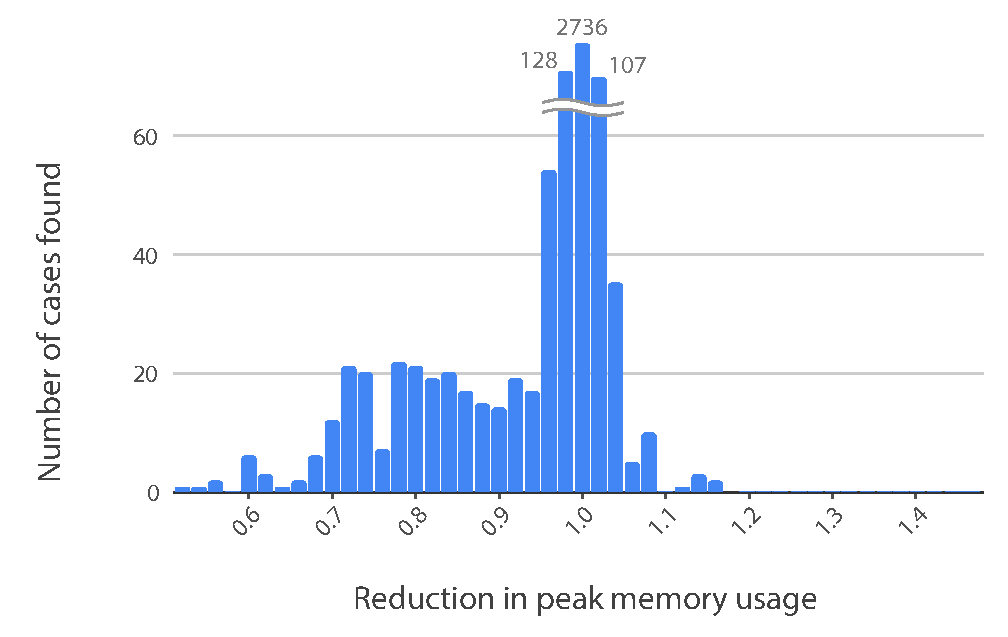
\includegraphics[width=4in]{figures/memoryhistogram.pdf}
\caption{Reduction in runtime peak memory usage of 3072 pieces of compiled
  code when 4127 synthesized rules are added to the TRS. The x-axis
  shows $\frac{after}{before}$, so below 1.0 means the synthesized rules
  reduced memory consumption.  In 197 cases,
  peak memory usage drops by more than 10\%.}
\label{fig:peakmemoryhistogram}
\end{figure*}

\paragraph{Term rewriting systems written without verification have bugs}
On our initial run of this experiment, 55 compilations (1.6\%) crashed
at runtime with memory corruption errors in the baseline condition (no
new rules added). We traced this to an incorrect transformation in a
separate, unverified TRS in the Halide compiler (the ``solver''). This
bug had existed for four years, but had only recently become an
important code path due to change $\mathbb{I}$ mentioned above. The
incorrect transformation was $\hmin(x - y, x - z) \rewrites x - \hmin(y, z)$,
which should be $\hmin(x - y, x - z) \rewrites x - \hmax(y, z)$. If this
secondary TRS had been written using verification, this bug would
never have been introduced. We intend to formalize and verify this
secondary TRS next to flush out any other bugs lurking therein.

\paragraph{The TRS scales well with the number of rules}
Remarkably, more than quadrupling the size of the TRS increased total compile
times by only 0.3\%. On further examination we found that the
additional rules increased the amount of time spent inside the TRS by
30\%, and that only 1\% of the the total compile time of the average
Halide program is spent inside the TRS.

We did not find significant effects on runtime of the generated code or code size. We also found no significant differences on any metrics within the Google corpus. This may be because the random schedules we generate are especially complex compared to human-written ones, or simply because humans don’t commit code that causes the compiler to misbehave.

While adding this many new rules does not come at any significant cost we could measure to users of Halide, it increases the compile-time and code size of the compiler itself, so we do not propose adding all of these rules to the TRS permanently. Prior to proposing inclusion, we plan to triage the rules to select only those that are necessary to gain the peak memory reductions described above.

These results show that having verification and synthesis available as a tool for compiler authors fixes existing bugs, prevents entire classes of new bugs, and even helps compiler writers change the semantics of their language with confidence. We intend to continue to use verification and synthesis to maintain the TRS, and based on this experience plan to expand its use elsewhere in the compiler.




% \begin{table*}

% \caption{Incorrect rules found during verification.}
% \begin{tabular}{l|l|l}
% Incorrect rule & Counterexample & Tool used \\
% \hline
% $((x + c_0)/c_1)*c_1 - x \rewrites x \bmod c_1 \textrm{ if } c_1 > 0 \wedge c_0 + 1 == c_1$ & x := -2, c_0 := 2, c_1 := 3 & Z3 \\
% $x - ((x + c_0)/c_1)*c_1 \rewrites -(x \bmod c_1) \textrm{ if } c_1 > 0 \wedge c_0 + 1 == c_1$ & x := -2, c_0 := 2, c_1 := 3 & Z3 \\
% $\hmin(x, c_0) < \hmin(x, c_1) + c_2 \rewrites \textrm{false if } c_0 >= c_1 + c_2)$ & x := 0, c_0 := 0, c_1 := -1, c_2 := 1 & Z3 \\
% $\hmax(x, c_0) < \hmax(x, c_1) + c_2 \rewrites \textrm{false if } c_0 >= c_1 + c_2$ & x := 0, c_0 := 2, c_1 := 1, c_2 := 1 & Z3 \\
% \end{tabular}
% \label{tab:incorrectrules}
% \end{table*}

\section{Limitations \& Future Work}
\label{sec:limitations}
For this work, we considered only the subset of the term rewriting system that
is used to prove properties over infinite integers; the full TRS includes rules
for simplifying expressions with floating point values as well as rules for
fixed-bitwidth integers.  As a result, we do not consider cases where the TRS
must also reason about whether overflow can occur.  Extending our improvements
and automation to such rules could be done in future work.

One major limitation of the synthesis process we use is that our oracle
for rules, Z3, often cannot reason about expressions with divisions or modulo
where the right operand is a variable.  Though we work around this to
synthesize rules with generalized predicates on right hand side constants,
the overall synthesis machinery cannot generalize these to non-constants.
Extending the synthesizer may be more tractable for rules that operate
on integers with finite bitwidths.

The Halide TRS is used both to prove expressions true or false and to
simplify expressions to more easily optimizable forms, but these two use cases
are not always aligned. One could imagine two separate rewriters with
different rulesets and reduction orders. One interesting direction for future
work might be to use the synthesizer to create these two rulesets, which would
otherwise be a very human-effort intensive task.

Although we do not currently synthesize rules that contain vector operators,
they are not incompatible with our approach. Since our reduction of Halide
expressions to SMT2 formulas models vector expressions as integers, we would need
to add a typechecking step to ensure correctness in the synthesis process, which
we leave as future work.

The priority in which rules are considered for matching clearly can have
performance implications, but evaluation and tuning is left as future work, and
may require modifying our ordering or creating different orderings for different
uses of the term rewriting system.

Finally, while enhancing the Halide TRS was not able to improve the performance of the mature Halide compiler, we suspect this may not be the case for other, less well-exercised compiler backends. In future work we plan to use this technique to enhance the ruleset used to compile Halide applications to GPU code or to the Hexagon ISA.

\section{Related Work}
Perhaps the closest related work is the Alive project~\cite{lopes2015alive,menendez2017aliveinfer}.
The fundamental difference between Alive and this
work is that Alive works within the decidable theory of bitvectors, while
(because of Halide semantics) we must use the undecidable theory of integers;
this constraint is the major reason for many of our design choices. In addition:
Alive verifies optimizations (and Alive-Infer synthesizes preconditions), while
we synthesize rewrites and predicates, as well as verify them; Alive must contend
with more types of undefined behavior, which the Halide expression
language need not consider; and Alive uses a simple reduction order in
which all optimizations reduce program size, while our termination proof is more
complex. We originally tried synthesizing rule predicates with the approach used
by Alive-Infer but were not successful: using Z3 to generate positive and
negative examples did not scale for us, requiring seconds to minutes per query
due to the underlying theory of integers.  Moreover, queries with
division/modulo over the integers often did not work at all, simply returning
``unknown.''

Most recently, leveraging a TRS along with synthesized rules has been applied
to optimizing fully-homomorphic encryption (FHE) circuits~\cite{lee2020fhe}.  This
system synthesizes equivalent circuits with lower cost from small example circuits,
then applies the equivalences in a divide-and-conquer manner; the rewrites do
not contain preconditions. In further contrast to our work, the domain of FHE yields a
simple cost function (the depth of nested multiplications in the circuit), and
the underlying theory of boolean circuits is decidable.


An \textit{equivalence graph} or egraph, as introduced by \citet{nelson1980techniques}, is a data structure used to compute applications of the rules of a term rewriting system. The algorithm builds up equivalence classes by successively applying all rules to all expressions within those classes, then queries to see if two expressions are equivalent by checking if they are present in the same class. Like our algorithm, it does not backtrack, but the egraph can require significant amounts of memory, which our algorithm avoids.

Herbie~\cite{panchekha2015automatically}, a tool for improving the accuracy of floating point arithmetic, uses an egraph term rewriting system made up of a small library of axioms to find repairs once a fault has been localized. Herbie assures termination by bounding the number of rewrites their system may apply, and achieves good performance by pruning the expression search space and applying rewrites only to particular expression nodes. 

Besides the closely-related projects described above, program synthesis has been applied to term rewriting systems in several domains. Swapper~\cite{singh2016swapper} synthesizes a set of rewrite rules to transform SMT formulas into forms that can be more easily solved by theory solvers, similar to the use of the Halide TRS as a simplifier, using the SKETCH tool. \citet{butler2017synthesizing} learns human-interpretable strategies (essentially rewrite rules) for puzzle games such as Sudoku or Nonograms and \citet{butler2018framework} finds tactics for solving K-12 algebra problems, both using a CEGIS loop similar to our synthesis process. None of these address termination, although Swapper likely screens out non-terminating rulesets through its autotuning step. The Butler works both focus on synthesizing small, highly general rulesets that are similar to human rewriting strategies, unlike the Halide TRS which tolerates very large rulesets. The \textbf{$\lambda^2$} tool~\cite{feser2015lambda} for example-guided synthesis performs inductive synthesis from examples, using a combination of inductive and deductive reasoning combined with enumerative search.  While our rewrite rules do not have the benefit of examples, it may be possible to apply this technique to obtain more sophisticated predicate synthesis for our rewrites.

Superoptimization, a process of finding a shorter or more desirable program that is semantically equivalent to a larger one, is similar to our work synthesizing right-hand side terms for candidate LHSs. STOKE~\cite{schkufza2013stochastic} uses Monte Carlo Markov Chain sampling to explore the space of x86 assembly programs, while \citet{phothilimthana2016scaling} describes a cooperative superoptimizer that searches for better programs using multiple techniques in a way that allows them to learn from each other.  Souper~\cite{sasnauskas2017souper} is a recent synthesis-based superoptimizer for LLVM, which was used as the basis for evaluating the effectiveness of Alive-Infer's{} precondition synthesis.

PSyCO~\cite{lopes2014weakest} synthesizes preconditions that guarantee a compiler optimization is semantics-preserving, using a counterexample-driven algorithm similar to our rule CEGIS loop (although not like our predicate synthesis algorithm). PSyCO finds the weakest precondition from a finite language of constraints, while the space of our predicate search is theoretically inifinite but in practice bounded by our iteration limit. PSyCO must reason about side effects by tracking read and write behavior in optimization templates, while our expression language is side effect-free. More recently, Proviso~\cite{astorga2019learning} finds preconditions for C\# programs using an active learning framework composed of a machine learning algorithm for decision trees as a black-box learner and a test generator that acts as a teacher providing counterexamples. Like this work, the logic of preconditions they synthesize is in an undecidable domain.

SMT solvers seek to achieve practical results in theoretically challenging problems, such as the theory of non-linear integer arithmetic. For example, \citet{jovanovic2017solving} describes a satisfiability procedure for NLIA that is effective in practice and implements it in the Yices2 solver. In this work we leverage Z3's NLIA solving abilities and extend synthesis to include certain types of non-linear expressions by using constants as operands and later generalizing.

\modified{A different use of term rewriting systems in pipeline scheduling language
compilers is demonstrated in \cite{hagedorn2020achieving}, in which an algorithm
and a schedule are rewritten using a TRS to low-level code, which can be then compiled
for high performance.}

\section{Conclusion}
\label{sec:conclusion}
In this work, we improved the Halide term rewriting system by applying formal
techniques to verify rewrite rules and to ensure termination.  In this process,
we discovered \NumRulesFixed incorrect rules (which is remarkable,
given that the TRS has been extensively fuzz tested) and \NumPredicatesRelaxed cases
where we could make rules more general, as well as \NumOrderingProblems rules
that could potentially cause termination problems.  We built
an automated synthesis-based pipeline for constructing new rewrite rules
and demonstrated that it can produce better rewrite rules than hand-authored ones
in five historical bug fixes. We further described four case studies in which the
synthesizer has served as an assistant to a human compiler engineer. Finally,
we showed that applying the synthesizer can proactively improve weaknesses
in the Halide compiler by bulk-synthesizing a large number of rules automatically
and demonstrating this ruleset lowers peak memory usage of compiled code with nearly
no increase in compilation time.
%from
%proof failures, augmenting the compiler with \NumRulesSynthesized synthesized
%rewrite rules and demonstrating that our system can be used to automatically fix
%user-reported compiler bugs.

Our improvements guarantee the soundness of the term rewriting system
and increase its robustness and coverage, with no significant costs or
downsides we could identify. Indeed, augmenting this part of the
Halide compiler using verification and synthesis seems to constitute a
free lunch, and so we intend to formalize other parts of the compiler as
verified term rewriting systems as well.


%% Acknowledgments
\begin{acks}                            %% acks environment is optional
                                        %% contents suppressed with 'anonymous'
  %% Commands \grantsponsor{<sponsorID>}{<name>}{<url>} and
  %% \grantnum[<url>]{<sponsorID>}{<number>} should be used to
  %% acknowledge financial support and will be used by metadata
  %% extraction tools.
This work was supported in part by the CONIX Research Center, one of six centers in JUMP, a Semiconductor Research Corporation (SRC) program sponsored by DARPA.
\end{acks}


%% Bibliography
\bibliography{bib}

\end{document}
